\documentclass[11pt,a4paper]{article}

% --- Packages
\usepackage[utf8]{inputenc}
\usepackage[T1]{fontenc}
\usepackage{amsmath, amssymb, amsthm, mathtools}
\usepackage{bm}
\usepackage{graphicx}
\usepackage{booktabs}
\usepackage{hyperref}
\usepackage[margin=1in]{geometry}
\usepackage{xcolor}
\usepackage{natbib}

% --- Theorem environments
\newtheorem{theorem}{Theorem}
\newtheorem{lemma}[theorem]{Lemma}
\newtheorem{corollary}[theorem]{Corollary}
\newtheorem{proposition}[theorem]{Proposition}
\theoremstyle{definition}
\newtheorem{definition}[theorem]{Definition}
\newtheorem{assumption}[theorem]{Assumption}
\theoremstyle{remark}
\newtheorem{remark}[theorem]{Remark}

% --- Custom macros
\newcommand{\R}{\mathbb{R}}
\newcommand{\E}{\mathbb{E}}
\newcommand{\norm}[1]{\left\lVert#1\right\rVert}
\newcommand{\inner}[2]{\left\langle#1,#2\right\rangle}
\newcommand{\loss}{\mathcal{L}}
\newcommand{\thetap}{\bm{\theta}}
\newcommand{\phip}{\bm{\phi}}
\newcommand{\EGR}{\mathrm{EGR}}
\newcommand{\Cg}{C_g}
\newcommand{\Cf}{C_f}
\newcommand{\TODO}[1]{\textcolor{red}{[TODO: #1]}}
\newcommand{\NOTE}[1]{\textcolor{blue}{[NOTE: #1]}}

% --- Title
\title{The Spectral Shortcut Theorem: A Gradient-Geometric \\
       Explanation for Failure Modes of Joint \\
       Spectral-Spatial Deep Learning}
\author{Krzysztof Dziuba \\ \texttt{krzys.dziuba@gmail.com}}
\date{\today}

\begin{document}
\maketitle

\begin{abstract}
\TODO{Write abstract last, after Phase 7.}
\end{abstract}

% --- Sections
\section{Introduction}
\label{sec:intro}

The integration of spectroscopic imaging with deep learning has produced
a class of compositional models that has become the de facto standard
across infrared tissue classification, hyperspectral remote sensing,
Raman imaging, and mass spectrometry imaging. A canonical pipeline
processes a hyperspectral input $X \in \R^{H \times W \times S}$ in two
stages: a per-pixel spectral reduction $f_\thetap: \R^S \to \R^K$
followed by a spatial model $g_\phip: \R^{K \times H \times W} \to
\R^{N_{\mathrm{cls}} \times H \times W}$. End-to-end joint training of
this pipeline is overwhelmingly the default — adopted by foundational
work in FTIR histology~\cite{berisha2019deep}, recent state-of-the-art
spatial-spectral ViTs for prostate tissue
classification~\cite{oleary2026spatial}, and essentially all
hyperspectral remote sensing systems.

\paragraph{An empirical paradox.}
Despite the prevalence of this paradigm, an unexpected and persistent
pattern has emerged across multiple subfields. Frozen pretrained
spectral encoders dramatically outperform end-to-end joint training
on held-out test data. In our motivating tissue classification setting,
a learned-from-scratch linear $f_\thetap$ trained end-to-end achieves
$0.675$ test F1; freezing a pretrained $f_\thetap$ yields $0.84$--$0.95$
test F1. Most strikingly, replacing $f_\thetap$ with \emph{frozen
random weights} yields $0.70$ test F1 --- outperforming the joint
trained model. Recent independent observations
\cite{oleary2026spatial,berisha2019deep} have noted, in different
terms, that aggressive spectral compression to $16$ features has
negligible impact on spatial-spectral neural network performance, and
have concluded that ``tissue classification only needs a small set of
spectral features.''

We argue the opposite. The reason end-to-end joint training fails is
not that spectral information is unimportant. It is that
\emph{end-to-end optimization fails to extract that information}, even
when the spectral signal is rich and discriminative. The problem is in
the training procedure, not the data.

\paragraph{This paper.}
We provide a rigorous explanation for the failure of joint
spectral-spatial training, grounded in the geometry of the loss
landscape and the dynamics of stochastic gradient descent on
compositional architectures with asymmetric capacity. Two main
theorems form our contribution.

\begin{itemize}
    \item \textbf{Theorem~\ref{thm:hessian} (Capacity-Induced Module
          Curvature Disparity).} We prove that the ratio of the
          spatial to the spectral Gauss-Newton block's top eigenvalue
          grows linearly with the spatial module's width $M$
          (equivalently, as $\sqrt{\Cg/\Cf}$ for architecture
          families with $\Cg = \Theta(M^2)$): as the spatial module
          widens, curvature concentrates in it while the spectral
          block's curvature stays capped by a width-independent
          constant. The proof is elementary: an explicit witness
          direction in the classifier-head weights forces the
          width-linear growth, and an operator-norm bound caps the
          spectral block; the rate matches the mean-field law of
          Karakida et al.~\cite{karakida2019universal} in the model
          class where the latter applies.
    \item \textbf{Theorem~\ref{thm:twoscale} (Finite-Time Spectral
          Starvation).} Under an explicit shortcut-fitting hypothesis
          compatible with cross-entropy dynamics, the spectral
          module's displacement from initialization by the time the
          training residual reaches level $\delta$ is at most
          $\mathcal{O}(\varepsilon \log(1/\delta))$, where
          $\varepsilon$ is the ratio of the (capped) spectral gradient
          scale to the shortcut fitting rate. As spatial capacity
          grows, the shortcut fits faster while the spectral gradient
          stays capped, so the spectral module is pinned near
          initialization for the entire useful duration of training.
          The formulation is finite-time by design: for unregularized
          cross-entropy on separable data no finite stationary point
          exists~\cite{soudry2018implicit}, and the starvation
          phenomenon is a training-time effect, not an asymptotic
          one.
\end{itemize}

\paragraph{A real-time diagnostic.}
The pathology described by Theorems~\ref{thm:hessian} and
\ref{thm:twoscale} is invisible to standard loss curves --- training
and validation loss both decay smoothly while the spectral module is
silently starved. To make the pathology observable in practice we
introduce the \emph{Effective Gradient Ratio} (EGR), a scalar
diagnostic computable inside any training loop:
\[
    \EGR(t) = \frac{\norm{\nabla_\thetap \loss(\thetap_t, \phip_t)}}
                   {\norm{\nabla_\phip \loss(\thetap_t, \phip_t)}}.
\]
Proposition~\ref{prop:egr_monotonic} establishes that the spectral
gradient norm---the EGR's numerator---decays polynomially while the
loss is being fitted. Empirically, the depth of the EGR collapse
scales monotonically with capacity ratio, providing a quantitative,
training-time observable for gradient starvation.

\paragraph{Prescription.}
The theory yields a direct prescription: freeze the spectral module,
or inject a fixed residual baseline. Freezing eliminates the timescale
gap by removing $\thetap$ from the optimization entirely. A residual
baseline ($Z = f_\thetap(X) + h(X)$ for a fixed $h$, e.g.\ PCA) is a
softer intervention that breaks the shortcut without precluding spectral
fine-tuning. We discuss both in Section~\ref{sec:discussion}.

\paragraph{Universality.}
Although our motivating application is infrared tissue classification,
the mechanism we identify applies to any compositional architecture
with capacity asymmetry between sequential modules. We verify in
Section~\ref{sec:experiments} that the same pattern manifests across
linear, CNN, and Vision Transformer spatial models on synthetic
hyperspectral problems, indicating the phenomenon is architecture-
agnostic. We expect the same mechanism to govern frozen-encoder
practices in Raman spectroscopy, mass spectrometry imaging, NIR
analysis, and beyond.

\paragraph{Relation to prior work.}
The closest prior work is in multimodal learning, where Wang et
al.~\cite{wang2020what} and Peng et al.~\cite{peng2022balanced}
identified ``modality competition'' and proposed gradient blending and
modulation interventions. Our setting is unimodal (a single
hyperspectral input) but the mechanism is structurally analogous: the
spatial and spectral subspaces of the input act as competing
``modalities,'' with the spatial module monopolizing the gradient
budget. We discuss this connection further in
Section~\ref{sec:related}.

\paragraph{Outline.}
Section~\ref{sec:related} reviews related work. Section~\ref{sec:setup}
establishes notation. Section~\ref{sec:thm1} proves
Theorem~\ref{thm:hessian}. Section~\ref{sec:thm2} proves
Theorem~\ref{thm:twoscale}. Section~\ref{sec:egr} formalizes the EGR
diagnostic. Section~\ref{sec:experiments} validates both theorems and
the diagnostic on synthetic spectral-spatial problems with linear, CNN,
and ViT spatial models. Section~\ref{sec:real} briefly connects the
synthetic findings to real FTIR/QCL tissue classification data.
Section~\ref{sec:discussion} discusses prescriptions, limitations, and
open problems.

\section{Related Work}
\label{sec:related}

Our analysis sits at the intersection of four lines of research: the
implicit bias and gradient dynamics of cross-entropy training; the
geometry of deep-network loss surfaces; multimodal gradient competition;
and spectral-spatial deep learning for biomedical and remote-sensing
applications. We survey each in turn.

\subsection{Gradient starvation and implicit bias}

Cross-entropy minimization is known to induce structural biases in the
learned representation. Soudry et al.~\cite{soudry2018implicit} proved
that on linearly separable data, gradient descent on logistic loss
converges to the maximum-margin classifier. Gunasekar et
al.~\cite{gunasekar2017implicit} and Lyu and Li~\cite{lyu2020gradient}
extended this picture to deep homogeneous networks. These results
establish that gradient-based training selects \emph{which} solution
among many that fit the training data.

Pezeshki et al.~\cite{pezeshki2021gradient} identified a distinct
phenomenon termed \emph{gradient starvation}: in the Neural Tangent
Kernel regime, dominant features in the input rapidly saturate the
cross-entropy loss, after which weaker but task-relevant features
receive negligible gradient signal. Our Theorem~\ref{thm:twoscale}
adapts this framework to compositional architectures, where the
``dominant features'' are introduced not by the input distribution
but by an architectural capacity asymmetry between modules. The
result is a module-level starvation rather than a feature-level one.

\subsection{Two-timescale stochastic approximation}

The classical machinery for analyzing coupled gradient flows with
disparate timescales is Borkar's stochastic approximation
framework~\cite{borkar2008stochastic}. Heusel et
al.~\cite{heusel2017gans} adapted this to neural network training by
introducing the Two Time-Scale Update Rule for GANs, proving
convergence to a local Nash equilibrium under explicit step-size
disparity. Our setting differs structurally: the timescale separation
in our compositional model is not imposed by the optimizer (the same
learning rate is applied to both modules) but emerges \emph{implicitly}
from the Hessian eigenvalue gap quantified by Theorem~\ref{thm:hessian}.

\subsection{Hessian geometry of deep networks}

The eigenspectrum of the neural-network Hessian has been characterized
empirically and theoretically. Sagun et al.~\cite{sagun2017empirical}
identified a bulk-plus-outliers structure for overparametrized
networks. Pennington and Bahri~\cite{pennington2017geometry} developed
a random matrix theory analysis that predicts spectral densities under
Gaussian assumptions. Karakida et al.~\cite{karakida2019universal}
derived closed-form mean-field expressions for the leading eigenvalue
of the Fisher Information Matrix, showing it scales with the layer
width and parameter count. Theorem~\ref{thm:hessian} applies these
results blockwise to the joint Hessian of a compositional model,
combining them with Schur complement bounds to yield a capacity-ratio
scaling for the joint condition number.

\subsection{Multimodal gradient competition}

The phenomenon most structurally analogous to ours is gradient
competition in multimodal learning. Wang, Tran, and
Feiszli~\cite{wang2020what} showed empirically that joint training of
multimodal classification networks underperforms unimodal training
because different modalities overfit and generalize at different
rates. They proposed Gradient Blending to dynamically reweight
modality-specific losses. Peng et al.~\cite{peng2022balanced}
identified ``modality laziness'' --- a tendency for one modality to
dominate training, leaving the other under-optimized --- and proposed
On-the-fly Gradient Modulation. These works are empirical; our
contribution adapts and extends their framework to the unimodal
\emph{compositional} setting and provides a rigorous geometric
foundation. The recent biomedical application of gradient blending
to multimodal sarcoma prognosis~\cite{bozzo2024multimodal} confirms
the mechanism operates in medical settings, but is restricted to
explicit dual-modality (MRI + clinical) architectures, not the
single-modality compositional pipelines we consider.

\subsection{Spectral-spatial deep learning}

Spectral-spatial deep learning has been an active area for over a
decade, primarily in two communities: biomedical infrared spectroscopy
and hyperspectral remote sensing. Berisha et al.~\cite{berisha2019deep}
established the benefit of combining spectral and spatial features for
FTIR histology and observed that some tissue types could be classified
from spatial features alone, with ``minimal chemical information''
required --- a foreshadowing of the spatial shortcut phenomenon we
diagnose. More recently, O'Leary et
al.~\cite{oleary2026spatial} systematically compared spatial-spectral
architectures for prostate cancer classification in infrared
spectroscopy and reported the striking finding that compressing the
spectral dimension to as few as 16 features had negligible effect on
all models tested. The authors interpreted this as evidence that
tissue classification requires only a limited spectral signature.
Our Theorem~\ref{thm:twoscale} provides an alternative explanation:
end-to-end training fails to extract the spectral signature even when
it is present.

The conceptually nearest work in biomedical imaging is the recent
characterization of shortcut learning in histopathology by Dawood and
Minhas et al.~\cite{dawood2026confounding}, who showed that AI models
predicting molecular biomarkers from H\&E images exploit spurious
correlations with clinicopathological features rather than learning
genuine biological signal. Our paper extends the shortcut-learning
framework into a new modality (spectroscopic imaging) with a different
mechanism (gradient competition driven by architectural asymmetry
rather than confounder leakage).

\subsection{Frozen and random features}

Frozen random features have a long history in machine learning. Saxe
et al.~\cite{saxe2011random} showed that convolutional networks with
random (untrained) filters achieve competitive performance on standard
benchmarks. Rahimi and Recht~\cite{rahimi2007random} established the
theoretical foundations of random features for kernel methods. More
recently, Coil and Cheney~\cite{coil2025freezing} showed that freezing
layers acts as implicit regularization in overparametrized networks.
These works establish that frozen random features are not an oddity
but a principled choice. Our contribution is to identify the specific
mechanism --- gradient starvation under capacity asymmetry --- under
which freezing is not merely competitive but \emph{strictly preferable}
to joint training.

\section{Setup and Preliminaries}
\label{sec:setup}

We analyze a generic two-module compositional model. While our motivating
application is infrared spectroscopic imaging for tissue classification,
the framework applies to any pipeline that first reduces a per-element
spectral signal and then applies a high-capacity spatial model. We
deliberately keep the notation domain-agnostic.

\subsection{The compositional model}

Let $X \in \R^{H \times W \times S}$ denote a hyperspectral input image,
where $H$ and $W$ are spatial dimensions and $S$ is the spectral
dimension.\footnote{Multi-channel inputs (e.g.\ raw absorbance together
with first and second derivatives) are handled by concatenating channels
along the spectral dimension; this changes only the input size and
leaves the analysis unaffected.} We write the per-pixel spectrum at
location $(h,w)$ as $x_{h,w} \in \R^S$.

The model consists of two modules applied sequentially:
\begin{enumerate}
    \item A \emph{spectral reduction} $f_\thetap: \R^S \to \R^K$
          applied independently to every pixel, producing a feature map
          $Z \in \R^{K \times H \times W}$ with
          $Z_{:,h,w} = f_\thetap(x_{h,w})$.
    \item A \emph{spatial model} $g_\phip: \R^{K \times H \times W} \to
          \R^{N_{\mathrm{cls}} \times H \times W}$ producing per-pixel
          class logits $\hat{y} = g_\phip(Z)$.
\end{enumerate}
We denote the composed model
$F_{\thetap,\phip}(X) = g_\phip(f_\thetap(X))$ and the parameter counts
$\Cf := \dim(\thetap)$ and $\Cg := \dim(\phip)$.

\begin{assumption}[Linear spectral reduction]
\label{ass:linear}
$f_\thetap$ is linear in $\thetap$: there exists $W \in \R^{S \times K}$
with $\thetap = \mathrm{vec}(W)$ and $f_\thetap(x_{h,w}) = W^\top x_{h,w}$.
\end{assumption}

\begin{remark}
Assumption \ref{ass:linear} captures the canonical case used widely in
spectroscopy pipelines, including the FTIR and QCL tissue
classification work we draw motivation from. It is also the cleanest
case in which the Hessian of $\loss$ admits closed-form block analysis.
We discuss extensions to shallow nonlinear $f_\thetap$ in
Section~\ref{sec:discussion} and verify empirically in
Section~\ref{sec:experiments} that the theorem's scaling persists when
$f_\thetap$ is replaced by a small MLP.
\end{remark}

\begin{assumption}[Spatial model regularity]
\label{ass:reg}
$g_\phip$ is twice continuously differentiable in $\phip$ with
$L$-Lipschitz gradients.
\end{assumption}

\begin{assumption}[Sub-Gaussian inputs]
\label{ass:subg}
Per-pixel inputs $\{x_{h,w}\}$ are sub-Gaussian with second moment
$\Sigma = \E[x_{h,w} x_{h,w}^\top]$ of bounded condition number.
\end{assumption}

\begin{assumption}[Capacity gap]
\label{ass:gap}
$\Cg / \Cf \to \infty$.
\end{assumption}

Assumption~\ref{ass:gap} is the structural condition under which our
theorems become informative. Empirically it is satisfied with several
orders of magnitude to spare in modern spectral-spatial architectures
(in our motivating example, $\Cg/\Cf \approx 325$).

\begin{assumption}[Bounded input Jacobian of the classifier]
\label{ass:inputlip}
There exists a constant $\widetilde{L} > 0$ depending on the depth of
$g_\phip$, the bottleneck dimension $K$, the number of classes
$N_{\mathrm{cls}}$, and the data distribution --- but \emph{not} on
the characteristic width $M$ or the total spatial parameter count
$\Cg$ --- such that
\[
    \sup_{\phip \in \Phi_{\mathrm{reg}},\ Z \in \mathcal{Z}_{\mathrm{reg}}}
    \left\| \frac{\partial g_\phip(Z)}{\partial Z} \right\|_{\mathrm{op}}
    \;\leq\; \widetilde{L},
\]
uniformly over the training-time parameter regime
$\Phi_{\mathrm{reg}}$ and the induced feature domain
$\mathcal{Z}_{\mathrm{reg}}$.
\end{assumption}

\begin{remark}[Why Assumption~\ref{ass:inputlip} is separate from Assumption~\ref{ass:reg}]
Assumption~\ref{ass:reg} bounds the second derivatives of $g_\phip$
with respect to \emph{parameters}~$\phip$ (the standard
$L$-smoothness condition of the optimization literature).
Assumption~\ref{ass:inputlip} bounds the first derivative with respect
to \emph{input features} $Z$---a different object with a different
constant. Parameter-side smoothness does not imply input-side
Lipschitzness; we require both.

At random Kaiming/Xavier initialization, the operator norm of a
variance-scaled random weight matrix is $\Theta(1)$ in width $M$ by
the Bai--Yin law~\cite{bai1993limit} (see also
Vershynin~\cite{vershynin2018high}, Thm.~4.4.5;
Marchenko--Pastur~\cite{marchenko1967distribution} describes the
corresponding bulk spectrum), giving
$\|\partial g_\phip/\partial Z\|_{\mathrm{op}} = \Theta(1)$ in width
$M$ for standard CNN and MLP blocks. Under the maximal-update
parameterization ($\mu$P) of Yang and
Hu~\cite{yang2021tensor}, the bound persists throughout training as
$M \to \infty$. Under standard-parameterization training with weight
decay $\lambda > 0$ and bounded-norm iterates,
Assumption~\ref{ass:inputlip} follows from the boundedness of
$\|\phip\|$ combined with the per-layer product-of-operator-norms
bound; the constant $\widetilde{L}$ depends multiplicatively on the
depth $L$ but not on the width. Softmax self-attention is Lipschitz
only on bounded inputs~\cite{kim2021lipschitz}, so
$\mathcal{Z}_{\mathrm{reg}}$ should be taken compact whenever
$g_\phip$ uses attention---this is guaranteed by LayerNorm before
attention, which is standard practice.
\end{remark}

\subsection{Loss and gradients}

We train with per-pixel cross-entropy:
\begin{equation}
\label{eq:loss}
    \loss(\thetap, \phip) = \frac{1}{HW} \sum_{h=1}^{H} \sum_{w=1}^{W}
    \mathrm{CE}\!\left( F_{\thetap,\phip}(X)_{:,h,w},\ y_{h,w} \right),
\end{equation}
where $y_{h,w} \in \{1, \dots, N_{\mathrm{cls}}\}$ is the ground-truth
class. Cross-entropy plays an essential role in
Section~\ref{sec:thm2}: its gradient with respect to the logits
$\hat{y}$ is the prediction residual
$r = \mathrm{softmax}(\hat{y}) - y_{\mathrm{onehot}}$, which vanishes
exponentially as predictions saturate. We discuss other loss functions
sharing this vanishing-residual property in
Section~\ref{sec:discussion}.

The gradient of $\loss$ with respect to the spatial parameters is
computed by standard backpropagation. The gradient with respect to the
spectral parameters $\thetap$ admits the chain-rule decomposition
\begin{equation}
\label{eq:chain}
    \nabla_\thetap \loss
    = \underbrace{\frac{\partial \loss}{\partial \hat{y}}}_{\text{residual}}
    \cdot \underbrace{\frac{\partial \hat{y}}{\partial Z}}_{\text{spatial Jacobian}}
    \cdot \underbrace{\frac{\partial Z}{\partial \thetap}}_{\text{input}}.
\end{equation}
The three factors play distinct roles in our analysis. The residual is
small when predictions are confident. The spatial Jacobian depends on
the current state of $\phip$ and thus changes throughout training. The
final factor is the input itself and is stationary. The product
structure implies that if the residual decays to zero, the gradient to
$\thetap$ vanishes regardless of the other two factors. This
observation underlies Theorem~\ref{thm:twoscale}.

\subsection{The block Hessian}

The joint Hessian of $\loss$ decomposes into blocks aligned with the
two parameter groups:
\begin{equation}
\label{eq:block_hessian}
    H = \nabla^2 \loss(\thetap, \phip) =
    \begin{pmatrix}
        H_{\thetap\thetap} & H_{\thetap\phip} \\
        H_{\phip\thetap} & H_{\phip\phip}
    \end{pmatrix},
\end{equation}
with $H_{\thetap\thetap} \in \R^{\Cf \times \Cf}$,
$H_{\phip\phip} \in \R^{\Cg \times \Cg}$, and cross blocks of
appropriate sizes. Theorem~\ref{thm:hessian} bounds the condition
number of $H$ in terms of $\Cg / \Cf$ by separately bounding the
spectrum of each block.

For optimization-rate analysis it is often more tractable to work with
the Gauss-Newton approximation $G = J^\top J$, where $J = [J_\thetap,
J_\phip]$ is the Jacobian of the per-pixel residuals. The two matrices
coincide near interpolation, and Theorem~\ref{thm:hessian} is stated
for $G$.

\subsection{The Effective Gradient Ratio}

We introduce a real-time diagnostic that tracks the asymmetry in
gradient flow between the two modules.

\begin{definition}[Effective Gradient Ratio]
\label{def:egr}
At training step $t$ with parameters $(\thetap_t, \phip_t)$, the
Effective Gradient Ratio is
\[
    \EGR(t) \;:=\; \frac{\norm{\nabla_\thetap \loss(\thetap_t, \phip_t)}}
                        {\norm{\nabla_\phip \loss(\thetap_t, \phip_t)}}.
\]
\end{definition}

\begin{remark}
EGR is a unitless quantity directly computable inside any training
loop with negligible overhead. Section~\ref{sec:egr} establishes its
monotonicity along the slow-fast manifold (a consequence of
Theorem~\ref{thm:twoscale}) and proposes a threshold criterion for
detecting gradient starvation onset.
\end{remark}

\subsection{Notational conventions}

Throughout, $\norm{\cdot}$ denotes the Euclidean ($\ell_2$) norm for
vectors and the spectral norm for matrices; $\lambda_{\max}(\cdot)$ and
$\lambda_{\min}(\cdot)$ denote the largest and smallest eigenvalues of
a symmetric matrix; $\kappa(A) = \lambda_{\max}(A)/\lambda_{\min}(A)$
its condition number. We write $A \succeq B$ to mean $A - B$ is
positive semidefinite. The symbol $\Omega(\cdot)$ is used in the
standard asymptotic sense.

\begin{definition}[Module curvature disparity]
\label{def:dcurv}
The \emph{module curvature disparity} of the joint Gauss-Newton
matrix is
\[
    \mathcal{D}_{\mathrm{curv}}(G)
    \;:=\; \frac{\lambda_{\max}(G_{\phip\phip})}
                {\lambda_{\max}(G_{\thetap\thetap})}
    \;=\; \frac{\lambda_{\max}(J_{\phip}^\top J_{\phip})}
                {\lambda_{\max}(J_{\thetap}^\top J_{\thetap})},
\]
the ratio of the spatial Gauss-Newton block's top eigenvalue to the
spectral block's top eigenvalue.
\end{definition}

\begin{remark}[Why disparity, not condition number]
\label{rem:disparity_vs_kappa}
Theorem~\ref{thm:hessian} is a purely geometric statement about how
curvature concentrates between the two modules as the spatial network
widens. It is not a joint-Hessian condition-number bound: the joint
Gauss-Newton $G$ is rank-deficient (parameter directions orthogonal
to the classifier's range have exactly zero curvature), so
$\kappa(G) = \lambda_{\max}(G)/\lambda_{\min}(G)$ is trivially
infinite. The disparity $\mathcal{D}_{\mathrm{curv}}$ is
well-defined regardless of rank structure, uses only well-behaved
operator-norm quantities, and is exactly the ratio measured in
Experiment~1.1. Its growth with spatial capacity is the geometric
mechanism that motivates the two-timescale dynamical analysis of
Theorem~\ref{thm:twoscale}, but the dynamical claim requires its own
hypotheses and does not follow from $\mathcal{D}_{\mathrm{curv}}$
alone.
\end{remark}

\section{Theorem 1: Capacity-Induced Module Curvature Disparity}
\label{sec:thm1}

This section establishes our first main result: the module curvature
disparity $\mathcal{D}_{\mathrm{curv}}$
(Definition~\ref{def:dcurv}) grows with the spatial module's width.
The result is the geometric foundation for the dynamical analysis of
Section~\ref{sec:thm2}: it identifies a capacity-dependent mechanism
capable of generating disparate module learning rates. The dynamical
starvation claim itself is stated separately in
Theorem~\ref{thm:twoscale}, under its own explicit hypotheses.

\subsection{Main result}

\begin{theorem}[Capacity-Induced Module Curvature Disparity]
\label{thm:hessian}
Consider the compositional model $F_{\thetap,\phip} = g_\phip \circ
f_\thetap$ with fixed-dimensional linear spectral module $f_\thetap$
(Assumption~\ref{ass:linear}) and a family of spatial networks
$g_\phip^{(M)}$ indexed by characteristic width $M$
(channels for a CNN, embedding dimension for a ViT, hidden width for
an MLP). Under
Assumptions~\ref{ass:linear}, \ref{ass:subg},
and~\ref{ass:inputlip}, together with the head
hypothesis of Lemma~\ref{lem:phi_scaling} below (a dense classifier
head over penultimate features of dimension $\Theta(M)$ that are
correlated across inputs at initialization), there exist
constants $c_1, c_2 > 0$ depending on the data distribution, the
initialization scheme, the bottleneck dimension $K$, the input
spectral dimension $S$, and the architecture class of $g_\phip$
(depth, activation, head dimensions)---but not on $M$ or on the
spatial parameter count $\Cg$---such that
\[
    \mathcal{D}_{\mathrm{curv}}^{(M)}
    \;=\; \frac{\lambda_{\max}(G^{(M)}_{\phip\phip})}
                {\lambda_{\max}(G_{\thetap\thetap})}
    \;\geq\; c_1 \cdot M - c_2
\]
in expectation over random Kaiming (variance-scaled Gaussian)
initialization. Equivalently, for architecture families with
$\Cg = \Theta(M^2)$,
\[
    \mathcal{D}_{\mathrm{curv}}^{(M)}
    \;\geq\; c_1' \cdot \sqrt{\Cg / \Cf} - c_2.
\]
\end{theorem}

\begin{remark}[Interpretation]
Theorem~\ref{thm:hessian} states that as the spatial network widens,
its top Gauss-Newton eigenvalue grows without bound while the
spectral module's top Gauss-Newton eigenvalue remains capped by a
$\Cg$-independent constant. Curvature increasingly concentrates in
the downstream module. This is a purely geometric fact about the
Hessian; the dynamical consequence---that joint training pins
$\thetap$ near its initialization---is stated separately in
Theorem~\ref{thm:twoscale}, under its own hypotheses. The disparity
measures the downstream module's \emph{readiness to move}---the
loss curvature its parameters command at initialization---not the
usefulness of its features: it is present before any feature has
been learned, and the width-linear spike can be exhibited even for
inputs carrying no information
(Remark~\ref{rem:instance_interpretation}, supplement). That the
geometry favours the spatial module \emph{independently} of feature
quality is precisely what makes it a shortcut hazard.
\end{remark}

The proof decomposes the disparity bound into separate bounds on the
top eigenvalues of the two diagonal blocks. We state the supporting
lemmas before presenting the proof.

\subsection{Supporting lemmas}

\begin{lemma}[Spatial block scaling]
\label{lem:phi_scaling}
Let $M$ denote the characteristic width of $g_\phip$ (channel count
for a CNN, embedding dimension for a ViT, hidden layer width for an
MLP), let $N_{\mathrm{cls}} \geq 2$, and suppose $g_\phip$ ends in a dense
classifier head over penultimate features
$h_n \in \mathbb{R}^{M_h}$ with $M_h = \Theta(M)$ whose
softmax-weighted mean Gram
$S_h^{p} := N^{-1}\sum_n p^{(n)}_{\min} h_n h_n^\top$
(Equation~\eqref{eq:feature_gram}) satisfies
\[
    \lambda_{\max}(S_h^{p}) \;\geq\; q_h M_h
    \quad\text{with probability } \geq 1 - \delta_h
\]
over the random initialization---where $p^{(n)}_{\min}$ denotes the
smallest softmax probability at pixel $n$---for constants $q_h > 0$
and $\delta_h < 1$ independent of $M$ (the \emph{head hypothesis}:
the features carry a common direction of $\Theta(M)$ energy across
inputs, on pixels whose initial predictions are non-degenerate. It
is a cross-input \emph{correlation} condition, not a per-vector norm
condition, and is closely related to the quantity $\kappa_2$
carrying the width-linear term in Karakida et al.'s
law---see the supplement, where a fully proved instance is also
given). Then the spatial Gauss-Newton
block of~\eqref{eq:ggn} satisfies
\[
    \lambda_{\max}(G_{\phip\phip})
    \;=\; \Omega(M)
    \qquad \parbox{15em}{\centering in expectation over random Kaiming
    (variance-scaled Gaussian) initialization.}
\]
The logit Gram $J_\phip^\top J_\phip \succeq G_{\phip\phip}$
inherits the bound unconditionally; the residual Gram
$J_\phip^{\mathrm{res}\top} J_\phip^{\mathrm{res}}$ satisfies it
under the analogous hypothesis on the $p^2$-weighted Gram
$S_h^{p^2}$ (supplement). For architecture families with
$\Cg = \Theta(M^2)$ (fixed depth with at least two consecutive
width-proportional layers), equivalently
$\lambda_{\max}(G_{\phip\phip}) = \Omega(\sqrt{\Cg})$.
\end{lemma}

\begin{remark}
Lemma~\ref{lem:phi_scaling} is proved in the supplement
(Section~\ref{sec:proof_thm1}) by an explicit witness: the rank-one
head-weight perturbation $V = c\, u^\top$, where $c$ is a unit class
contrast and $u$ the dominant direction of the feature ensemble.
Evaluating the curvature along $V$ gives the deterministic
inequality $\lambda_{\max}(G_{\phip\phip}) \geq
\lambda_{\max}(S_h^{p})$, and the head hypothesis supplies
$\lambda_{\max}(S_h^{p}) = \Omega(M)$. The
width-linear law agrees with the mean-field analysis of Karakida et
al.~\cite{karakida2019universal}: their Theorem~4 gives
$\lambda_{\max} = \Theta(M)$ with sharp constant for
proportional-width fully connected networks under squared loss, and
their Theorem~1 shows the mean eigenvalue simultaneously shrinks as
$\mathcal{O}(1/M)$---curvature concentrates in a vanishing fraction
of directions as networks widen. The scaling variable is width, not
parameter count: for architecture families with $\Cg = \Theta(M^2)$,
the equivalent parameter-count statement is
$\lambda_{\max} = \Omega(\sqrt{\Cg})$. The head hypothesis covers
per-pixel dense heads on CNN and ViT modules as well; the sharpness
of the width-linear rate is tested empirically in
Section~\ref{sec:experiments}.
\end{remark}

\begin{lemma}[Spectral block operator-norm cap]
\label{lem:opcap}
Under Assumptions~\ref{ass:linear} (linear per-pixel $f_\thetap$),
\ref{ass:subg} (bounded input second moment), and~\ref{ass:inputlip}
(bounded input Jacobian
$\|\partial g_\phip / \partial Z\|_{\mathrm{op}} \leq \widetilde{L}$
uniformly in $\Cg$), the spectral logit Jacobian and Gauss-Newton
block satisfy
\[
    \lambda_{\max}(G_{\thetap\thetap})
    \;\leq\; \|J_\thetap\|_{\mathrm{op}}^{2}
    \;\leq\; \widetilde{L}^{2} \cdot \lambda_{\max}(\Sigma_X)
    \;=:\; C_\thetap,
\]
where $C_\thetap$ depends only on the classifier's input Lipschitz
constant $\widetilde{L}$ and the top eigenvalue of the mean per-pixel
input Gram $\Sigma_X$ of~\eqref{eq:sigma_x}---not on the spatial
width $M$, the spatial parameter count $\Cg$, or the dataset size
$N$. The same bound holds for the residual-Gram convention, since
$H_\tau^2 \preceq H_\tau \preceq I$.
\end{lemma}

\begin{remark}
Lemma~\ref{lem:opcap} follows from the chain-rule identity
$J_\thetap = J_Z \cdot (\partial Z / \partial \thetap)$ for the logit
Jacobian, combined with $\|J_Z\|_{\mathrm{op}} \leq \widetilde{L}$
(Assumption~\ref{ass:inputlip}) and the exact form of $\partial Z /
\partial \thetap$ under linearity of $f_\thetap$
(Assumption~\ref{ass:linear}, giving the per-pixel factor $I_K
\otimes x_n^\top$, whose $N$-normalized stacking has
$\|\partial Z / \partial \thetap\|_{\mathrm{op}}^{2} =
\lambda_{\max}(\Sigma_X)$ exactly, by
$I_K \otimes \Sigma_X$). Passing from the logit Jacobian to the
Gauss-Newton block or the residual Jacobian only inserts factors of
$H_\tau \preceq I$ and can only decrease the bound. The bound is on
the operator norm (equivalently, the top eigenvalue), which is
well-behaved under rank-deficiency of the block---avoiding the
smallest-eigenvalue and Kronecker-factorisation machinery discussed
in Section~\ref{sec:proof_thm1}.
\end{remark}

\subsection{Proof of Theorem~\ref{thm:hessian}}

\begin{proof}[Proof of Theorem~\ref{thm:hessian}]
By Lemma~\ref{lem:phi_scaling}, in expectation over random Kaiming
(variance-scaled Gaussian) initialization,
\[
    \lambda_{\max}(G^{(M)}_{\phip\phip}) \;\geq\; c_\phi \cdot M
\]
for a constant $c_\phi > 0$ independent of $M$ (depending on the
initialization scheme, the activation, the head dimensions, and the
data distribution; supplement Section~\ref{sec:proof_thm1}). By
Lemma~\ref{lem:opcap},
\[
    \lambda_{\max}(G_{\thetap\thetap})
    \;\leq\; \|J_\thetap\|^2_{\mathrm{op}} \;\leq\; C_\thetap
\]
for a constant $C_\thetap > 0$ independent of $M$. The cap is
deterministic---it holds for every realization of the
initialization---so it may be divided through inside the
expectation:
\[
    \E\!\left[\mathcal{D}_{\mathrm{curv}}^{(M)}\right]
    \;=\; \E\!\left[\frac{\lambda_{\max}(G^{(M)}_{\phip\phip})}
                {\lambda_{\max}(G_{\thetap\thetap})}\right]
    \;\geq\; \frac{\E\!\left[\lambda_{\max}(G^{(M)}_{\phip\phip})\right]}
                  {C_\thetap}
    \;\geq\; \frac{c_\phi \cdot M}{C_\thetap}
    \;=\; c_1 \cdot M
\]
with $c_1 := c_\phi / C_\thetap$. The witness route delivers the
bound with $c_2 = 0$; the subtracted constant is retained in the
statement so that sharper asymptotic constants, valid only for
large $M$, may be substituted. Under
$\Cg = \Theta(M^2)$ (families with at least two consecutive
width-proportional layers), $M = \Theta(\sqrt{\Cg})$
and the ratio form $c_1' \cdot \sqrt{\Cg / \Cf}$ follows on multiplying
and dividing by $\sqrt{\Cf}$. This completes the proof.
\end{proof}

\subsection{Implications}

Theorem~\ref{thm:hessian} establishes that curvature concentrates in
the downstream spatial module as its width grows. We highlight two
implications, and separate them explicitly from the dynamical
consequences of Section~\ref{sec:thm2}.

\paragraph{Geometric mechanism, not a dynamical claim.}
$\mathcal{D}_{\mathrm{curv}} \gg 1$ identifies a
\emph{potential} for disparate module learning rates: the spatial
Gauss-Newton block admits directions of arbitrarily large curvature
while the spectral block does not. Whether joint gradient descent
actually produces disparate effective learning rates depends on an
additional dynamical hypothesis (that the shortcut pathway fits the
residual at rate $\mu$; Assumption~\ref{ass:residual}), which
Section~\ref{sec:thm2} introduces and Experiment~1.2 tests.
Theorem~\ref{thm:hessian} does not,
by itself, prove that $\thetap$ is pinned to initialization.
In particular, $\mathcal{D}_{\mathrm{curv}}$ concerns the \emph{top}
of the spatial block's spectrum, while the fitting rate $\mu$ of
Section~\ref{sec:thm2} is governed by how fast the residual can be
driven down---a property of other parts of the spatial spectrum. The
two are linked only under spectral-shape assumptions we do not make;
the theorems are deliberately independent, and
Experiments~1.1--1.2 test them separately.

\paragraph{The disparity is invariant to shared step-size tuning.}
The disparity bound depends only on architectural parameters, not on
the choice of optimizer or the shared step-size schedule---so no
choice of shared learning rate changes the \emph{geometry}; whether
any shared-step-size method escapes the \emph{dynamical} consequence
is a separate question we treat as a conjecture below. Adaptive
methods (Adam, RMSProp) rescale per-coordinate gradient magnitudes
but do not alter the underlying eigenvalue disparity between the two
blocks. Two-timescale optimizers with explicitly different learning
rates per module (Heusel et al.~\cite{heusel2017gans}; Borkar
2008~\cite{borkar2008stochastic} Ch.~6) are the natural remedy at the
optimizer level. We discuss this in Section~\ref{sec:discussion}.

\subsection{Relation to classical ill-conditioning}
\label{sec:classical_conditioning}

Ill-conditioned optimization has classical causes with classical
remedies, and it is natural to ask whether they apply here. They do
not, because the disparity of Theorem~\ref{thm:hessian} is driven by
the \emph{architecture}, not by the data or the parametrization of a
single block.

\paragraph{Feature normalization.}
Scale asymmetry or collinearity among input features degrades the
conditioning of $\Sigma_X$ and is classically cured by
standardizing (e.g.\ mean-centering) the inputs. Here the cure has
a sharper, quantitative role: Lemma~\ref{lem:opcap} places
$\lambda_{\max}(\Sigma_X)$ in the spectral cap, so input
transformations that deflate the top of the input spectrum
\emph{raise} the realized disparity at every width---normalization
moves the constants. What no input transformation can touch is the
width-scaling of the spatial block (Lemma~\ref{lem:phi_scaling}):
capacity moves the rate. On raw nonnegative spectra, whose second
moment is dominated by the shared mean shape, the cap is large and
the realized disparity correspondingly small; mean-centering is
predicted to restore it (Section~\ref{sec:real}).

\paragraph{Weight decay.}
Adding $\alpha \norm{w}^2$ to the loss shifts the Hessian by
$2\alpha I$, lifting every eigenvalue by $2\alpha$ and famously
repairing classical condition numbers. But the shift acts on
\emph{both} blocks equally: the disparity becomes
$(\lambda_{\max}(G_{\phip\phip}) + 2\alpha) /
(\lambda_{\max}(G_{\thetap\thetap}) + 2\alpha)$, which remains
$\Theta(M)$ for any fixed $\alpha$ as $M$ grows. Repairing the
disparity would require $2\alpha \sim \lambda_{\max}(G_{\phip\phip})$,
a regularization strength that would dominate the data term and
prevent fitting. Consistent with this, Experiment~1.6 finds that
Pezeshki's Spectral Decoupling---an $L_2$ penalty on logits designed
to combat saturation---does not reduce the joint-training collapse,
while freezing does.

\paragraph{Adaptive optimizers.}
Adam and RMSProp precondition per-coordinate gradient magnitudes with
a diagonal rescaling. The raw block spectra are
optimizer-invariant, but the \emph{dynamics} under a diagonal
preconditioner $P$ are governed by the preconditioned spectra of
$P^{-1/2} G P^{-1/2}$ and need not respect the disparity: under
Adam, per-coordinate steps are near-constant in gradient magnitude,
so small spectral gradients do not imply small spectral movement.
The gradient-flow statements of Section~\ref{sec:thm2} are
accordingly scoped to (stochastic) gradient descent; joint-vs-frozen
gaps observed under Adam are evidence about the phenomenon, not
applications of the theorem. Empirically, the
canonical dynamics experiment (Experiment~1.2) is run under Adam and
the joint-vs-frozen gap persists at every width; we treat the stronger
claim---that no shared-learning-rate adaptive method can remove the
pathology---as a conjecture rather than a theorem. Optimizers with
explicitly different learning rates per module (two-timescale update
rules; Heusel et al.~\cite{heusel2017gans}) are the natural remedy at
the optimizer level and correspond, in the limit, to our freezing
prescription.

\begin{remark}[Parameterization scope]
\label{rem:param_scope}
$\mathcal{D}_{\mathrm{curv}}$ is not invariant to per-module
reparameterization, and Theorem~\ref{thm:hessian} is a statement
about the standard variance-scaled (Kaiming) parameterization---the
one used in the pipelines we analyze and in all our experiments.
Under alternative parameterizations that rescale layers with width,
such as $\mu$P~\cite{yang2021tensor}, both the initialization
magnitudes and the effective per-layer learning rates change, and
the width scaling of the blocks would need to be re-derived; we do
not claim the disparity law transfers. Our two uses of $\mu$P
elsewhere are limited to a different role: as one route to keeping
the input-Jacobian bound (Assumption~\ref{ass:inputlip}) uniform in
width during training. Whether principled reparameterization can
neutralize the disparity---rather than merely re-expressing it---is
an open question adjacent to the per-module learning-rate remedies
discussed in Section~\ref{sec:discussion}.
\end{remark}

\begin{remark}[Small eigenvalues: irrelevance vs.\ starvation]
\label{rem:irrelevance_vs_starvation}
A parameter direction can carry vanishing curvature for two very
different reasons: (a) the direction genuinely does not affect
predictions on the task at hand (``irrelevance''), in which case zero
gradient is the correct outcome and the parameter should not be
learned; or (b) the direction \emph{would} affect predictions if the
optimizer could reach it, but the compositional geometry buries the
gradient signal behind the bottleneck (``starvation''). The
Gauss-Newton bounds of Theorem~\ref{thm:hessian} alone cannot
distinguish between these interpretations: both produce
$\Cg$-independent small curvature in the spectral block.

The synthetic experiments in Section~\ref{sec:experiments} are
designed to distinguish these hypotheses by construction. In
Experiment~1.3 we generate data where each of the two modalities alone
carries information sufficient to solve the task (single-modality
baselines reach $\approx 0.53$ on a binary classification, above the
$0.50$ chance floor). Joint training on the same data does not merely
under-use the spectral channel: it undershoots the weaker of the two
single-modality baselines. The gap is modest in absolute terms on this
synthetic problem---an important honest caveat---but its direction is
inconsistent with interpretation~(a), under which joint training
would at worst match the stronger single-modality baseline.

For real spectroscopic data, distinguishing (a) from (b) requires
demonstrating that a frozen pretrained spectral encoder outperforms
one that has been jointly trained end-to-end on the same task. We
report such experiments on FTIR and QCL tissue classification in
Section~\ref{sec:real}. Our present study compares only two
concrete mitigation strategies (freezing the spectral module, and
Pezeshki's Spectral
Decoupling~\cite{pezeshki2021gradient}); broader comparisons against
modality-specific learning rates, gradient surgery, GradNorm-style
loss balancing, and related interventions are important future work.
\end{remark}

\subsection{Empirical support}

Experiment~1.1 in Section~\ref{sec:experiments} measures
$\mathcal{D}_{\mathrm{curv}}^{(M)}$ directly across a range of
spatial widths and confirms monotonic growth with $M$: the spatial
top eigenvalue grows $74\times$ over the sweep while the spectral
top eigenvalue stays flat, driving the disparity into the thousands.
The measured log--log slope of $\lambda_\phi$ against $\Cg$ is
$0.70 \pm 0.05$, below the slope-$1.0$ prediction that applies to
the tested architecture family (whose $\Cg = \Theta(M)$); the
deficit and its candidate causes are reported in
Section~\ref{sec:experiments}. The qualitative
prediction---unbounded spatial-block growth against a capped
spectral block---is unambiguous in the data.

\begin{remark}[Defense against linear triviality]
\label{rem:not_pca}
A natural objection is that, since $f_\thetap$ is linear, the analysis
must reduce to principal component analysis (PCA) of the input. This
is not the case. PCA finds directions of maximum input variance
\emph{without reference to labels}. At initialization, however, the
distinction is limited, and we state this candidly: the
Gauss--Newton blocks carry no label information there (the softmax
weights are near-uniform), and $G_{\thetap\thetap}$ is, by
Lemma~\ref{lem:opcap}, an input-second-moment object propagated
through a label-free random network. The defense against
PCA-triviality is therefore a statement about \emph{training}: along
the trajectory the supervised residual shapes
$\partial \hat{y}/\partial Z$ and hence the curvature, and the
pathology we identify is precisely that this supervised signal
fails to reach $\thetap$---not that $f_\thetap$ is incapable of
representing useful features.
\end{remark}

\section{Theorem 2: Finite-Time Spectral Starvation}
\label{sec:thm2}

Theorem~\ref{thm:hessian} is a geometric statement: as the spatial
module widens, curvature concentrates in it and the spectral block's
top curvature stays capped. This section states the dynamical
consequence we actually observe in training---the spectral module
barely moves during the period in which the training loss is being
fit---as a theorem with \emph{explicit dynamical hypotheses}. We
deliberately do not claim that the geometry of
Theorem~\ref{thm:hessian} alone implies the dynamics: the bridge from
curvature disparity to rate separation is stated as a hypothesis,
motivated by Theorem~\ref{thm:hessian} and verified empirically in
Section~\ref{sec:experiments}. Deriving it from the architecture is
left as an open problem (Section~\ref{sec:discussion}).

Two classical facts shape the formulation. First, for unregularized
cross-entropy on separable data there is \emph{no finite minimizer}:
the loss decays like $1/t$ while the parameters diverge along the
max-margin direction (Soudry et al.~\cite{soudry2018implicit}).
A theorem asserting convergence to a finite stationary point would
therefore be vacuous or false in the regime modern networks inhabit.
Second, the starvation phenomenon of Pezeshki et
al.~\cite{pezeshki2021gradient} is fundamentally about which features
receive learning signal \emph{during training}, not about the
$t \to \infty$ limit. Both point the same way: the honest statement is
a \emph{finite-time} bound on how far the spectral parameters can move
before the shortcut pathway has fitted the labels.

\subsection{Setting and hypotheses}

We analyze the continuous-time limit of joint training with a shared
learning rate, in which the parameters $(\thetap_t, \phip_t)$ evolve
by gradient flow
\begin{equation}
\label{eq:gf}
    \dot{\thetap}(t) = -\nabla_\thetap \loss(\thetap, \phip),
    \qquad
    \dot{\phip}(t) = -\nabla_\phip \loss(\thetap, \phip).
\end{equation}
The discrete-SGD extension (Robbins--Monro tracking with noise
entering the constants) is standard
(Borkar~\cite{borkar2008stochastic}, Ch.~2) and discussed in the
supplement.

Recall from the chain rule~\eqref{eq:chain} that
$\nabla_\thetap \loss = J_\thetap^\top r$ where $r$ is the softmax
residual, so
\begin{equation}
\label{eq:theta_grad_bound}
    \norm{\dot{\thetap}(t)}
    \;=\; \norm{J_\thetap(t)^\top r(t)}
    \;\leq\; \norm{J_\thetap(t)}_{\mathrm{op}} \cdot \norm{r(t)}.
\end{equation}
Fix a horizon $T > 0$ and suppose the trajectory remains in the
regime of Assumption~\ref{ass:inputlip}, i.e.\
$\phip(t) \in \Phi_{\mathrm{reg}}$ and $Z(t) \in
\mathcal{Z}_{\mathrm{reg}}$ for all $t \leq T$
(\emph{trajectory containment}). Under
Assumptions~\ref{ass:linear}, \ref{ass:subg},
and~\ref{ass:inputlip}, Lemma~\ref{lem:opcap} then caps the first
factor over that horizon:
\begin{equation}
\label{eq:bt}
    B_T \;:=\; \sup_{t \leq T} \norm{J_\thetap(t)}_{\mathrm{op}}
    \;\leq\; \sqrt{C_\thetap}
    \;=\; \widetilde{L}\,\sqrt{\lambda_{\max}(\Sigma_X)},
\end{equation}
a constant independent of the spatial width $M$, the parameter count
$\Cg$, and the horizon $T$. (Even without containment,
$B_T < \infty$ for every finite $T$ by continuity of $J_\thetap$
along the flow; containment is what makes the cap
\emph{$M$-independent}, which is the load-bearing property.) We write
$B$ for $B_T$ when the horizon is clear. The remaining hypothesis
concerns the second factor.

\begin{remark}[Containment and the unregularized separable regime]
\label{rem:containment}
Trajectory containment is a genuine restriction. In the
unregularized separable regime that motivates the polynomial
envelope below, $\norm{\phip(t)} \to \infty$ logarithmically
(Soudry et al.~\cite{soudry2018implicit}), so a bound on
$\|\partial g_\phip/\partial Z\|_{\mathrm{op}}$ that is uniform over
\emph{all} $t$ cannot be assumed. Two standard settings restore it:
weight decay or norm constraints (bounded iterates), and the
maximal-update parameterization~\cite{yang2021tensor} (bound uniform
in width). In the pure max-margin limit, $\widetilde{L}$ grows at
most logarithmically in $T$, which turns the displacement bound of
Theorem~\ref{thm:twoscale} into
$\mathcal{O}(\varepsilon \log^2(1/\delta))$---the same conclusion up
to a log factor.
\end{remark}

\begin{assumption}[Shortcut residual decay]
\label{ass:residual}
There exist constants $C \geq 1$ and $\mu > 0$ such that, along the
joint trajectory~\eqref{eq:gf},
\[
    \norm{r(t)} \;\leq\; \frac{C}{1 + \mu t},
\]
where $\norm{r(t)}$ is the root-mean-square per-pixel residual
of~\eqref{eq:jacobians}. We refer to $\mu$ as the \emph{shortcut
fitting rate}. The constants $C$ and $\mu$ may depend on the
initialization, the data, and the architecture---in particular
$\mu$ is expected to grow with spatial capacity
(Remark~\ref{rem:residual_motivation})---and are not assumed uniform
over any family; the theorem holds for any trajectory admitting such
an envelope.
\end{assumption}

\begin{remark}[Why polynomial, and where $\mu$ comes from]
\label{rem:residual_motivation}
The $1/t$ envelope is the correct cross-entropy-compatible form: for
logistic-type losses on separable data the training loss---and hence
the residual norm---decays polynomially, not exponentially
(Soudry et al.~\cite{soudry2018implicit}). An exponential envelope,
where valid (e.g.\ regularized or non-separable regimes), only
strengthens the conclusion below. The hypothesis encodes the
\emph{shortcut} mechanism: the residual is driven down by the spatial
module exploiting whatever signal is present in the feature map $Z$
(positional and contextual structure), without requiring $f_\thetap$
to specialize---the spatial-signal sufficiency discussed in
Section~\ref{sec:thm2_hypotheses}. The rate $\mu$ is expected to
\emph{grow} with spatial capacity: wider networks fit faster (in the
NTK regime, the fitting rate is governed by the spatial kernel's
smallest relevant eigenvalue, which grows with width; see
Pezeshki et al.~\cite{pezeshki2021gradient}). We verify this
empirically in Experiment~1.2, where time-to-fit shrinks monotonically
with $D$. A derivation of $\mu(\Cg)$ for the linearized fast subsystem
is given informal treatment in the supplement and is not needed for
the theorem, which takes $\mu$ as given.
\end{remark}

\begin{definition}[Fitting time]
\label{def:fitting_time}
For a target residual level $\delta \in (0, C)$, the fitting time is
\[
    T_\delta \;:=\; \inf\{\, t \geq 0 : \norm{r(t)} \leq \delta \,\}.
\]
Under Assumption~\ref{ass:residual}, $T_\delta \leq (C/\delta - 1)/\mu$.
\end{definition}

\subsection{Main result}

\begin{theorem}[Finite-Time Spectral Starvation]
\label{thm:twoscale}
Fix a horizon $T \geq 0$ and suppose the gradient flow~\eqref{eq:gf}
is contained in $\Phi_{\mathrm{reg}} \times
\mathcal{Z}_{\mathrm{reg}}$ up to time $T$. Under
Assumptions~\ref{ass:linear}, \ref{ass:subg}, \ref{ass:inputlip},
and~\ref{ass:residual}, with $B_T$ as in~\eqref{eq:bt}, the flow
satisfies
\[
    \norm{\thetap(T) - \thetap_0}
    \;\leq\; \frac{B_T\,C}{\mu} \, \log(1 + \mu T),
\]
and, whenever $T \geq T_\delta$, at the fitting time $T_\delta$,
\[
    \norm{\thetap(T_\delta) - \thetap_0}
    \;\leq\; \frac{B_T\,C}{\mu} \, \log\!\left(\frac{C}{\delta}\right).
\]
In particular, writing $\varepsilon := B_T/\mu$ for the effective
module-rate ratio, the spectral displacement by the time the training
residual reaches level $\delta$ is
$\mathcal{O}\!\left(\varepsilon \log(1/\delta)\right)$.
\end{theorem}

\begin{proof}
By~\eqref{eq:theta_grad_bound}, the operator-norm cap~\eqref{eq:bt},
and Assumption~\ref{ass:residual}, for every $t \leq T$,
\[
    \norm{\dot{\thetap}(t)}
    \;\leq\; B_T \cdot \norm{r(t)}
    \;\leq\; \frac{B_T\,C}{1 + \mu t}.
\]
Integrating,
\[
    \norm{\thetap(T) - \thetap_0}
    \;\leq\; \int_0^T \norm{\dot{\thetap}(t)}\, dt
    \;\leq\; B_T\,C \int_0^T \frac{dt}{1 + \mu t}
    \;=\; \frac{B_T\,C}{\mu} \log(1 + \mu T).
\]
For the second claim, Definition~\ref{def:fitting_time} gives
$1 + \mu T_\delta \leq C / \delta$, so $\log(1 + \mu T_\delta) \leq
\log(C/\delta)$.
\end{proof}

\subsection{Interpretation}

Theorem~\ref{thm:twoscale} is a statement about \emph{training-time}
behavior, which is what practice cares about: training runs end when
the loss is fit (or by early stopping), not at $t = \infty$.

\paragraph{The starvation regime.}
The displacement bound is the product of two factors with opposite
capacity dependence. The numerator $B$ is capped independently of
$\Cg$ (Lemma~\ref{lem:opcap}): no matter how large the spatial module,
the spectral gradient cannot exceed $B \norm{r}$. The fitting rate
$\mu$ grows with spatial capacity
(Remark~\ref{rem:residual_motivation}): wider shortcut pathways
drive the residual down faster. Hence $\varepsilon = B/\mu \to 0$ as
capacity grows, and the spectral module is increasingly pinned to its
initialization \emph{for the entire useful duration of training}. This
is the capacity-worsens-starvation prediction verified in
Experiment~1.2, where the joint-vs-frozen gap grows monotonically with
$D$.

\paragraph{What we do not claim.}
We make no claim about the $t \to \infty$ limit. For unregularized
cross-entropy on separable data no finite stationary point exists
(Soudry et al.~\cite{soudry2018implicit}), and $\thetap$ may
eventually move substantially over horizons exponentially longer than
any practical training run ($T = \mathcal{O}(\varepsilon^{-q})$ still
yields displacement $\mathcal{O}(\varepsilon \log(1/\varepsilon)) \to
0$, but larger horizons are unconstrained). The finite-time framing is
not a weakness: it is the phenomenon. A spectral module that receives
its learning signal only after the loss has been fitted receives it
too late to shape which features the classifier uses.

\paragraph{The logarithm is benign.}
For any polynomial training horizon $T = \mathcal{O}(\varepsilon^{-q})$
with fixed $q$, the displacement is
$\mathcal{O}(\varepsilon \log(1/\varepsilon))$, which vanishes as
$\varepsilon \to 0$. The bound is thus meaningful across every
practically reachable horizon, not merely at a single stopping time.

\subsection{On the hypotheses}
\label{sec:thm2_hypotheses}

\paragraph{The operator-norm cap is proven, not assumed.}
The factor $B$ is supplied by Lemma~\ref{lem:opcap} under
Assumptions~\ref{ass:linear} and~\ref{ass:inputlip}; it is the point
where Theorem~\ref{thm:hessian}'s geometry genuinely enters the
dynamics.

\paragraph{Residual decay encodes the shortcut.}
Assumption~\ref{ass:residual} requires the training residual to fall
at rate $\mu$ \emph{without} the spectral module specializing. This is
plausible exactly when the spatial model can interpolate the training
labels from the structure already present in $Z$ (positional cues,
contextual patterns)---the spatial-signal sufficiency condition. In
practice it is satisfied whenever the spatial model can overfit the
training set, which is the norm for modern over-parameterized CNNs and
ViTs. We verify it empirically in Experiments~1.2 and~1.3: joint
training reaches near-zero training loss while the spectral module
remains close to initialization.

\paragraph{Rate separation is motivated, not derived.}
Theorem~\ref{thm:hessian} shows curvature disparity grows with
capacity; it does not by itself prove that $\mu$ grows or that the
trajectory satisfies Assumption~\ref{ass:residual}. We keep the two
theorems logically independent: Theorem~\ref{thm:hessian} identifies a
capacity-dependent geometric mechanism \emph{capable} of generating
disparate module learning rates; Theorem~\ref{thm:twoscale}
characterizes the starvation dynamics \emph{when} such a separation is
present. Experiments~1.1--1.3 test the mechanism and the dynamics
separately. Deriving Assumption~\ref{ass:residual} from the
architecture (e.g.\ via an NTK analysis of the fast subsystem at large
width, adapting Pezeshki et al.~\cite{pezeshki2021gradient}) is a
natural next step; a sketch is given in the supplement.

\TODO{Supplement: (i) discrete-SGD extension of
Theorem~\ref{thm:twoscale} via Robbins--Monro tracking
(Borkar Ch.~2), noise entering the constants; (ii) informal NTK
derivation of $\mu(\Cg)$ for the linearized fast subsystem;
(iii) empirical verification that $\norm{r(t)}$ on our synthetic
trajectories is enveloped by $C/(1+\mu t)$.}

\section{The Effective Gradient Ratio Diagnostic}
\label{sec:egr}

Theorems~\ref{thm:hessian} and~\ref{thm:twoscale} together identify a
training pathology that is invisible to standard loss curves: as
cross-entropy decays toward zero on both training and validation
sets, the spectral module is silently gradient-starved. A practitioner
running joint training sees the loss go down and the validation
accuracy go up, with no in-training signal that the spectral module
has failed to specialize. The implication for held-out test
performance is only revealed once test data is examined---often after
many epochs of wasted compute, or after deployment.

This section introduces the \emph{Effective Gradient Ratio} (EGR), a
real-time diagnostic that detects gradient starvation as it occurs.
EGR is a single scalar, computable inside any training loop at
negligible cost, that converts the finite-time starvation prediction
of Theorem~\ref{thm:twoscale} into a concrete observable.

\subsection{Definition and basic properties}

Recall from Definition~\ref{def:egr} that at training step $t$,
\[
    \EGR(t) = \frac{\norm{\nabla_\thetap \loss(\thetap_t, \phip_t)}}
                   {\norm{\nabla_\phip \loss(\thetap_t, \phip_t)}}.
\]
The numerator and denominator are computable directly from gradients
accumulated during the standard backward pass. EGR is unitless and
invariant to the choice of learning rate.

\paragraph{Initial value: a heuristic.}
A useful rule of thumb for the starting point of the diagnostic is
\begin{equation}
\label{eq:egr_init}
    \EGR(0) \;\sim\; \sqrt{\Cf / \Cg}
    \qquad \text{(heuristic, not a theorem).}
\end{equation}
The reasoning is a parameter-counting one: at variance-scaled
initialization each module's gradient has entries of comparable
typical magnitude, so the squared gradient norms scale with the
number of parameters carrying them,
$\norm{\nabla_\phip \loss}^2 \sim \Cg$ against
$\norm{\nabla_\thetap \loss}^2 \sim \Cf$, and the square root comes
from passing to norms. We state~\eqref{eq:egr_init} as a heuristic
rather than a proposition for three reasons: it exchanges the
expectation of a ratio for the ratio of expectations without a
concentration argument; the per-entry-magnitude premise is
parametrization-dependent and would change under $\mu$P, which we
cite elsewhere~\cite{yang2021tensor}; and the spectral module's
gradient additionally passes through the bottleneck, which the count
ignores. Its role in this paper is limited to setting the scale for
the \emph{relative} threshold of Definition~\ref{def:alert}, which
compares $\EGR(t)$ against the measured $\EGR(0)$ of the run at hand
and so does not depend on~\eqref{eq:egr_init} being sharp. The
corresponding numerical value for our motivating architecture follows
from the capacity ratio reported in Section~\ref{sec:real}.

\subsection{Decay of the spectral gradient}

\begin{proposition}[Spectral gradient decay]
\label{prop:egr_monotonic}
Under the hypotheses of Theorem~\ref{thm:twoscale}
(Assumptions~\ref{ass:linear}, \ref{ass:inputlip},
and~\ref{ass:residual}),
\[
    \norm{\nabla_\thetap \loss(t)}
    \;\leq\; \frac{B\,C}{1 + \mu t},
\]
where $B$ is the operator-norm cap of Lemma~\ref{lem:opcap} and
$C, \mu$ are the constants of Assumption~\ref{ass:residual}.
\end{proposition}

\begin{proof}
By the chain rule~\eqref{eq:chain},
$\norm{\nabla_\thetap \loss} \leq \norm{J_\thetap}_{\mathrm{op}}
\norm{r} \leq B \norm{r}$, and Assumption~\ref{ass:residual} bounds
$\norm{r(t)}$.
\end{proof}

\begin{remark}[From gradient decay to the EGR ratio]
\label{rem:egr_ratio_caveat}
Proposition~\ref{prop:egr_monotonic} bounds the \emph{numerator} of
the EGR. The denominator $\norm{\nabla_\phip \loss} =
\norm{J_\phip^\top r}$ is also proportional to the residual, so both
quantities vanish together as the loss is fitted, and the behavior of
their ratio is not determined by residual decay alone: it depends on
the relative conditioning of the two Jacobians along the trajectory.
We therefore treat the EGR trajectory as an empirical object,
characterized in Section~\ref{sec:egr-empirical}, and use
Proposition~\ref{prop:egr_monotonic} only for the absolute claim that
the spectral module's learning signal decays polynomially while the
loss is being fitted.
\end{remark}

\subsection{Threshold criterion}

Proposition~\ref{prop:egr_monotonic} suggests a practical criterion
for detecting the onset of gradient starvation.

\begin{definition}[Gradient starvation alert]
\label{def:alert}
We say the model is in a \emph{gradient starvation regime} at step $t$
if
\[
    \EGR(t) \;\;<\;\; \tau \cdot \EGR(0),
\]
where $\tau \in (0, 1)$ is a user-supplied tolerance. Empirically, we
recommend $\tau \in [0.05, 0.1]$, corresponding to a 10--20$\times$
drop in EGR relative to initialization.
\end{definition}

\begin{remark}
The threshold $\tau$ is the only hyperparameter of the diagnostic.
The default $\tau = 0.1$ corresponds to a one-decade decay and is the
value we use throughout Section~\ref{sec:experiments}. We provide a
sensitivity analysis to $\tau$ in the supplement.
\end{remark}

\paragraph{Practical use.}
A practitioner logs $\EGR(t)$ at each step. When the alert fires,
two options are available:
\begin{enumerate}
    \item \textbf{Freeze the spectral module.} This is the prescription
          most directly motivated by Theorem~\ref{thm:twoscale}:
          removing $\thetap$ from the optimization eliminates the
          timescale gap. We discuss this in Section~\ref{sec:discussion}.
    \item \textbf{Inject a fixed residual baseline.} A softer
          intervention: replace $Z = f_\thetap(X)$ with
          $Z = f_\thetap(X) + h(X)$ for a fixed feature extractor
          $h$ (e.g.\ PCA). The fixed baseline ensures the spatial
          model receives stable input even if $f_\thetap$ continues
          to drift, breaking the shortcut without freezing.
\end{enumerate}
We evaluate both interventions in Experiment~1.3.

\subsection{Relationship to existing diagnostics}

EGR is conceptually related to several existing notions but is
distinct in its scope and intent.

\paragraph{GradNorm~\cite{chen2018gradnorm}.}
GradNorm dynamically reweights losses in multi-task learning to
equalize gradient magnitudes across tasks. EGR measures rather than
intervenes, and applies to single-task compositional architectures
rather than multi-task losses.

\paragraph{Modality-specific learning rates (MSLR).}
In multimodal learning, MSLR adjusts learning rates per modality. EGR
diagnoses the underlying pathology that MSLR addresses but in a
unimodal, two-stage architecture where the ``modalities'' are
the spectral and spatial subspaces of a single input.

\paragraph{Loss curve monitoring.}
The conventional practice of monitoring training and validation loss
fails to detect gradient starvation because both can decay even as
$\thetap$ stagnates. EGR is sensitive to the structural failure
even when no global loss curve abnormality is present.

\subsection{Empirical validation: EGR as a diagnostic}
\label{sec:egr-empirical}

We validate EGR as a diagnostic of training pathology in two stages.
First, we establish that EGR statistics correlate with generalisation
across our full sweep. Second, we test whether the signal is genuine
or merely a re-encoding of model capacity.

\paragraph{Pooled correlation (capacity confounded).}
Across $N=24$ runs spanning four widths $\{16,64,256,1024\}$ with six
seeds each, EGR depth correlates strongly with final test accuracy:
Pearson $r = -0.723$ ($p = 6.6\times 10^{-5}$), Spearman $\rho = -0.808$
($p = 1.8\times 10^{-6}$), and with the train--test gap at $r = +0.741$
($p = 3.5\times 10^{-5}$). However, EGR depth is itself strongly
correlated with $\log\mathrm{width}$ ($r = +0.903$): roughly $77\%$ of
the pooled correlation with test accuracy is attributable to capacity
rather than to EGR depth per se (partial $r$ controlling for
$\log\mathrm{width}$ collapses to $-0.169$, $p = 0.44$). The pooled
correlation alone cannot establish a capacity-independent diagnostic.

\paragraph{Fixed-capacity test.}
To isolate the capacity-independent signal, we ran a second experiment
holding CNN width fixed at $D = 256$ and varying data noise
$\{0.05,0.10,0.15,0.20\}$, learning rate
$\{3{\times}10^{-4},10^{-3},3{\times}10^{-3}\}$, weight decay
$\{0,10^{-3}\}$, and six seeds, for a total of $N = 144$ runs. At fixed
capacity, $\mathrm{EGR}_{\min}$ is the relevant statistic (with width
fixed, $\mathrm{egr\_depth}$ reduces to a constant offset of
$\mathrm{egr\_min}$ in expectation). It exhibits a within-capacity
correlation with generalisation that is statistically robust but
practically moderate: Pearson $r(\mathrm{EGR}_{\min}, \mathrm{acc}) =
+0.344$ ($p = 2.5\times 10^{-5}$).

The relationship survives every adversarial control we applied.
$\mathrm{EGR}_{\min}$ is essentially orthogonal to the swept
hyperparameters --- marginal correlations with noise, learning rate,
and weight decay are $+0.029$, $-0.073$, and $+0.007$ respectively,
with the full hyperparameter set explaining only $R^{2} = 0.015$ of
$\mathrm{EGR}_{\min}$ variance. The partial correlation
$r(\mathrm{EGR}_{\min}, \mathrm{acc} \mid \mathrm{noise}, \mathrm{lr},
\mathrm{wd}) = +0.395$ ($p = 9.5\times 10^{-7}$) is \emph{larger} than
the pooled $r = +0.334$, which is the opposite signature of a hidden
hyperparameter confound. The within-bin analysis is the strongest
evidence: across the 24 $(\mathrm{noise}, \mathrm{lr}, \mathrm{wd})$
cells in which only the seed varies, 23 of 24 yield strongly positive
$r(\mathrm{EGR}_{\min}, \mathrm{acc})$ (mean $+0.584$, Fisher-$z$
aggregated $t = 14.65$, $p < 10^{-13}$).

Controlling for final training loss --- itself a non-trivial predictor
with $r = +0.47$ for accuracy and $r = -0.55$ for the overfit gap ---
leaves the $\mathrm{EGR}_{\min}$ partial correlation essentially
unchanged at $+0.335$ ($p = 4.1\times 10^{-5}$). EGR therefore carries
information that train-loss monitoring does not.

\paragraph{Practical interpretation.}
Honesty about effect size is required. Treated as a binary alarm,
$\mathrm{EGR}_{\min}$ achieves ROC-AUC $= 0.612$ for flagging
below-median test accuracy, and $\mathrm{EGR}_{\mathrm{depth}}$
achieves only $0.538$ for high overfit gap. The best operating point
($\mathrm{EGR}_{\min} < 0.10$) catches $90\%$ of bad runs but also
flags $57\%$ of healthy runs --- no threshold delivers a usable
trade-off as a standalone indicator.

\paragraph{Verdict.}
At fixed capacity, EGR is a real, capacity-independent signal
correlated with generalisation. The within-capacity effect size is
small enough that EGR is best deployed alongside train-loss monitoring
as a complementary diagnostic, not as a standalone run-quality
indicator. For research and ablation work, EGR provides genuine
insight into the gradient starvation mechanism beyond what loss
monitoring reveals; for production monitoring of single training
runs, plain loss curves remain the primary signal and EGR a useful
adjunct.

\subsection{Implementation}

The EGR diagnostic is implemented as a PyTorch training callback. It
hooks into the standard training loop between the backward pass and
the optimizer step:
\begin{verbatim}
loss.backward()
egr_logger.log_step(global_step)   # <-- the only added line
optimizer.step()
optimizer.zero_grad()
\end{verbatim}
The callback identifies the spectral and spatial parameter groups via
\verb|model.spectral.parameters()| and \verb|model.spatial.parameters()|
(or any user-supplied naming convention) and records the gradient
norms and EGR at each step. We release the implementation as the
\verb|egr| package, available at the project repository.
\TODO{Phase 4, W12: prepare PyPI package skeleton. Add unit tests
for gradient norm computation and threshold detection.}

\section{Synthetic Experiments}
\label{sec:experiments}

\TODO{Phase 5 (W13-W15). Four experiments validating the theorems.}

\subsection{Experiment 1.1 — Capacity ablation}
\TODO{Vary $\Cg / \Cf$, measure $\kappa(H)$ via power iteration. Predict slope $\approx 1$ on log-log.}

\subsection{Experiment 1.2 — Two-timescale dynamics}
\TODO{Fixed capacity ratio. Track loss, $\norm{\nabla_\thetap \loss}$, $\norm{\nabla_\phip \loss}$, EGR.}

\subsection{Experiment 1.3 — The equal-information experiment}
\TODO{Calibrate synthetic data so $I(y; h_s) = I(y; h_l)$. Five conditions show joint training collapses to spatial-only despite equal information.}

\subsection{Experiment 1.4 — EGR as predictor}
\TODO{20 model variants, correlate early-epoch EGR with final test F1.}

\section{Real-Data Study: Geometry, Dynamics, and Scope}
\label{sec:real}

The synthetic experiments in Section~\ref{sec:experiments} verify the
theorems where their assumptions hold. This section takes the theory to
a production-scale spectral-spatial pipeline: per-pixel 4-class tissue
classification on QCL infrared hyperspectral images of breast cancer
tissue microarrays. It contains two kinds of evidence with two distinct
roles. First, a production-scale \emph{observation} from a companion
empirical study \citep{dziuba2026spatial}: end-to-end training of the
spectral module loses badly to pretraining and freezing it. Second, a
\emph{controlled, instrumented study} on the same data and architecture
family, designed to test the theorems' predictions directly --- with
matched arms, logged gradient dynamics, and the optimizer family varied
across momentum SGD and AdamW. The picture that emerges is more
qualified than simple confirmation: the block-scalar reading of
Theorem~\ref{thm:hessian} does \emph{not} manifest at initialization,
for a reason we can measure (rank-one input statistics); a strong
directional curvature anisotropy is measurable at initialization,
and whether it starves learning is a hypothesis we state and test; the
momentum-SGD controls, which vary the optimizer family but do not
instantiate Theorem~\ref{thm:twoscale}'s gradient flow, show no
resolvable best-validation difference between joint and frozen arms at
three seeds; and the joint-versus-frozen comparison turns out to depend
on the training
protocol rather than on the architecture --- under our original
protocol it inverts between checkpoint policies, and under a protocol
that equalizes the incidental asymmetries between the arms neither a
freezing benefit nor a freezing penalty is resolvable at three seeds.

\subsection{Pipeline and capacity}
\label{sec:real_setup}

The data are $336 \times 336$ pixel cores collected by QCL
spectroscopy over the $1000$--$1800$~cm$^{-1}$ fingerprint region.
Each pixel carries an $S = 942$ dimensional spectrum (after stacking
raw absorbance and its first two derivatives). The classification
target is per-pixel tissue type. The compositional model is the Block
Vision Transformer of O'Leary et al.~\cite{oleary2026spatial}: a
linear per-pixel $f_\thetap: \R^{942} \to \R^{K}$, then $16 \times 16$
patch tokenization, a 12-layer / 12-head Vision Transformer of
embedding width $M = 192$, a transposed-convolution decoder, and a
convolutional segmentation head. Parameter counts obtained directly
from the instantiated model are given in Table~\ref{tab:capacity}.

\begin{table}[h]
\centering
\caption{Module capacities of the BlockViT-v2 pipeline, counted from
the instantiated model. $K$ is the spectral bottleneck width; the two
rows are the two configurations used in the companion's production
runs.}
\label{tab:capacity}
\begin{tabular}{lrrr}
\toprule
Configuration & $\Cf$ & $\Cg$ & $\Cg/\Cf$ \\
\midrule
$K = 64$ (end-to-end baseline) & $61{,}108$ & $18{,}271{,}540$ & $299$ \\
$K = 128$ (matched to frozen variants) & $121{,}588$ & $21{,}472{,}564$ & $177$ \\
\bottomrule
\end{tabular}
\end{table}

\paragraph{Channel convention.}
O'Leary et al.'s original BlockViT operates on the second-derivative
spectrum alone (a single channel, $S = 965$ for their prostate FTIR
data)---the field-standard preprocessing in infrared histopathology.
The companion benchmark, and hence the models analyzed here, instead
stacks raw absorbance with its first two derivatives (three channels,
$S = 942$). The choice affects only $\Cf$: instantiating the same
model on the single-channel field-standard input gives
$\Cf = 20{,}916$ and $\Cg/\Cf \approx 874$. The three-channel
convention is therefore the \emph{conservative} choice for this
paper's purposes---under the field standard, the capacity asymmetry
we analyze is roughly three times larger.

The capacity ratio is thus roughly two orders of magnitude, and the
spatial module's dominant blocks---the transformer
($5.34 \times 10^6$) and the transposed convolution
($9.44 \times 10^6$)---are both $\Theta(M^2)$ in the embedding width.

\paragraph{The architecture does not satisfy Theorem~\ref{thm:hessian}'s
head hypothesis.}
That $\Theta(M^2)$ scaling is not sufficient to place the model inside
the theorem. BlockViT-v2's segmentation head is the chain
$\mathrm{Conv}_{3\times3}(M{+}K \to 96) \to \mathrm{BN} \to
\mathrm{ReLU} \to \mathrm{Conv}_{3\times3}(96 \to 48) \to \mathrm{BN}
\to \mathrm{ReLU} \to \mathrm{Conv}_{3\times3}(48 \to 4)$, so the final
affine classifier sees $48 \times 3 \times 3 = 432$ input features at
\emph{every} width we build ($M \in \{48,192,384\}$,
$K \in \{64,128\}$): the $\Theta(M)$ feature map is separated from the
logits by two nonlinearities. Theorem~\ref{thm:hessian} requires a
dense classifier head over penultimate features of dimension
$\Theta(M)$ with no downstream nonlinearity
(Lemma~\ref{lem:phi_scaling}), and that hypothesis is therefore not
satisfied here; the $\Cg = \Theta(M^2)$ form of the statement is a
change of variables conditional on the same hypothesis, not an
independent sufficient condition. The theorem's lower bound on the
curvature disparity consequently does not apply as stated to this
model. This is different from the theorem being contradicted: failing a
hypothesis removes a guarantee, it does not reverse the conclusion.
Whether the curvature disparity the theorem permits actually manifests
at initialization is an empirical question, which we now measure
directly.

\subsection{Production-scale observation}
\label{sec:real_observation}

The companion study trains the full pipeline under 5-fold
cross-validation on breast QCL data and reports held-out test macro-F1
for an end-to-end learned linear spectral module against three
pretrain-and-freeze variants (its Table~6):

\begin{table}[h]
\centering
\begin{tabular}{lc}
\toprule
Variant & Test F1 (5-fold mean $\pm$ sd) \\
\midrule
End-to-end learned linear (joint)          & $0.675 \pm 0.036$ \\
Frozen pretrained spectral (Peak Windows)  & $0.842 \pm 0.121$ \\
Frozen pretrained spectral (MLP)           & $0.896 \pm 0.092$ \\
Frozen pretrained spectral (Sliding Win.)  & $0.954 \pm 0.020$ \\
\bottomrule
\end{tabular}
\caption{Held-out test F1 on breast QCL tissue cores, as published in
the companion study \citep{dziuba2026spatial}. End-to-end training of
the spectral module underperforms every pretrain-and-freeze variant by
$0.17$--$0.28$ F1.}
\label{tab:real}
\end{table}

Two remarks on scope. First, this is an \emph{observation that
motivates the controlled study below}, not a theorem test: the
variants differ in both stability (frozen vs.\ jointly trained) and
informativeness (pretrained vs.\ learned from scratch), and the
production runs log no gradient dynamics. Second, the theorems do not
guarantee that pretrain-and-freeze wins. Theorem~\ref{thm:twoscale}
bounds how far the spectral module moves along the \emph{joint}
trajectory in its regime; it does not by itself bound the performance
gap to a separately trained frozen model, and pretraining is a
separate, empirically supported escape route. The controlled study
below examines exactly these factors.

\subsection{Geometry at initialization}
\label{sec:real_geometry}

We measure the Gauss--Newton blocks of the instantiated pipeline on
real training batches at random initialization (Lanczos with full
reorthogonalization on matrix-free GGN block operators, validated to
$10^{-12}$ against dense computation; Section~\ref{sec:experiments}),
sweeping the ViT embedding width $M \in \{48, 96, 192, 384\}$ with
3 seeds $\times$ 4 batches per width.

\paragraph{The block-scalar disparity does not manifest.}
At production width $M=192$ the measured curvature ratio is
$\mathcal{D}_{\mathrm{curv}} = \lambda_{\max}(G_{\phip\phip})/\lambda_{\max}(G_{\thetap\thetap})
= 0.46 \pm 0.21$ --- the \emph{spectral} block carries the larger top
curvature, the opposite of the naive block-scalar expectation. The
ratio rises with width ($0.33 \pm 0.12$ at $M{=}48$ to
$0.70 \pm 0.19$ at $M{=}384$; on prostate QCL it reaches parity,
$1.09 \pm 0.52$, at $M{=}384$) but the disparity regime is nowhere in
sight at buildable widths. The two width-scalings behave differently.
The spectral cap is width-independent, as Theorem~\ref{thm:hessian}
requires (log-log slope of $\lambda_{\max}(G_{\thetap\thetap})$ vs.\ $M$:
$-0.003$ breast, $-0.012$ prostate). The spatial curvature grows, but
sublinearly: the log-log slope of $\lambda_{\max}(G_{\phip\phip})$ vs.\
$M$ is $0.38$ (breast) and $0.45$ (prostate), i.e.\ $115 \to 258$
across an $8\times$ width increase, well short of the $\Omega(M)$
growth of Lemma~\ref{lem:phi_scaling}. That $\Omega(M)$ floor is
neither observed here nor, given the head hypothesis failure noted in
Section~\ref{sec:real_setup}, guaranteed for this architecture.

\paragraph{What carries the width trend.}
The sublinear growth of $\lambda_{\max}(G_{\phip\phip})$ is measurable at
initialization, and it is not the mechanism of
Lemma~\ref{lem:phi_scaling}. In BlockViT-v2 the only downstream layer
whose input dimension grows with $M$ is the first head convolution, and
the second-moment matrix of the (patch-unfolded) features entering it is
flat in $M$: its top eigenvalue is unchanged to four significant figures
across $M \in \{48, 192, 384\}$ (3 seeds), with the leading direction
inside the width-independent $K{=}64$ skip channels. At initialization,
the positive width trend in the decoder's spatial GGN is sensitive to head
batch normalization: using fixed initial statistics in the two head BNs
removes the trend while preserving the incoming features (pooled log-log
slope of the first-convolution block's top curvature: $+0.61$ with batch
statistics, per seed $+0.35$ to $+0.79$; $+0.006$ with both head BNs at
their initial running statistics, per seed $-0.11$ to $+0.18$; whole
$\phip$ block $+0.40 \to -0.33$), and either BN alone carries it ($+0.56$
and $+0.57$). The mechanism is a normalization gain on width-diluted
activations. Under fan-in initialization the per-channel pre-BN variance
of the first head BN falls as $1/(M{+}K)$ ($0.15, 0.064, 0.035$ at the
three widths; medians over channels, 3 seeds), because the fan-in grows
with $M$ while the incoming energy sits almost entirely in the
width-independent skip channels; the BN's inverse-standard-deviation gain
grows correspondingly ($2.6, 4.0, 5.4$), so a unit weight perturbation
whose pre-BN energy is width-independent leaves the BN with energy growing
roughly as $M^{1/2}$ (measured slopes $0.46$--$0.56$) and reaches the loss
as $M^{0.6}$. A spatially constant bias perturbation is annihilated
exactly. A function-preserving rescaling of that convolution (weights and
bias by $c$, BN stabilizer by $c^2$) leaves every logit unchanged and
scales the block's top curvature by exactly $c^{-2}$ (measured $1.0000$
for $c \in \{\tfrac14, \tfrac12, 2, 4\}$), so the raw Euclidean curvature
of a layer that feeds a batch normalization is a parameterization
quantity, not an architectural one \citep{vanlaarhoven2017l2}. This sweep
therefore does not validate the width-linear feature-Gram mechanism of our
shallow theory, and we do not use it as architectural evidence. Slopes
over three widths are descriptive; the interventions establish
sensitivity, not a unique cause, since switching a BN to fixed statistics
also changes its forward output and the gates downstream of it. The
denominator, by contrast, we can diagnose directly.

\paragraph{Diagnosis: rank-one input statistics.}
The input second-moment matrix $\Sigma_X$ of real tissue spectra has
effective rank $1.07$ (breast) and $1.02$ (prostate) out of $942$ on
the raw inputs; measured after the module's input batch normalization
the same quantity is $1.21$ (breast), so the near-rank-one structure is
a property of the spectra and not an artifact of the normalization.
Every tissue spectrum shares the same dominant mean shape, and the cap
$C_\theta \propto \lambda_{\max}(\Sigma_X)$ is correspondingly enormous.
Theorem~\ref{thm:hessian}'s disparity bound is not established for this
model (its head hypothesis fails); independently, rank-one inputs make
the cap side uninformative: even where the bound applies, it constrains
nothing at buildable widths, because the data concentrate almost all
their second-moment mass in one direction. This is a regime in which
the scalar bound is uninformative, not a counterexample: the theorem's
disparity is a statement about what capacity \emph{permits}, and
rank-one inputs hand the spectral block a single direction of huge
curvature.

\paragraph{Directional curvature anisotropy.}
Because the spectral curvature is rank-deficient, the block-scalar
ratio is the wrong lens; restricting the GGN to individual directions
reveals an anisotropy the scalar hides. Write $v_1$ for the leading
eigenvector of the post-normalization input second-moment matrix; it
coincides with the mean-spectrum direction ($|\cos| > 0.995$
post-normalization, $> 0.9999$ on the raw inputs). Three measurements,
all at initialization. First, the $\thetap$-block top eigenvector,
matricized over the spectral projection weights, places
$0.954 \pm 0.017$ of its norm in the $K$-dimensional subspace induced
by $v_1$ (a subspace-projection fraction, not a vector cosine).
Second, the top $40$ of $61{,}108$ spectral directions hold
$0.83 \pm 0.12$ of the trace (per seed $0.69$--$1.00$, $n=3$). Third,
along the component of the clinically decisive CancerEpi--CAS class
contrast that is orthogonal to $v_1$ --- a component retaining
$76$--$84\%$ of the contrast's squared norm --- the restricted
curvature is $12$--$28\times$ smaller than along $v_1$ itself
(3 seeds $\times$ 3 batches at $M{=}192$). The curvature along the
\emph{un-orthogonalized} full contrast --- which retains its $v_1$
component ($|\cos(d, v_1)| = 0.45$) --- the gap is far smaller:
$3.7\times$ on average (range $2.6$--$4.8$; 3 seeds $\times$ 3 batches).
The large ratio is therefore a statement about the $v_1$-orthogonal part
of the contrast; along the contrast as a whole the anisotropy is modest.
Meanwhile the
spatial
block's top eigenvalue overtakes the spectral spectrum already at rank
$2$--$5$ (Figure~\ref{fig:real_geometry}). On the strength of this
geometry we \emph{hypothesize} that the gradient signal available for
learning discriminative spectral features --- as opposed to re-encoding
the mean spectrum --- is suppressed relative to the mean direction, and
we test that hypothesis against the training dynamics of
Section~\ref{sec:real_dynamics}. The geometry on its own establishes
the anisotropy, not its consequence for learning.

\begin{figure}[t]
\centering
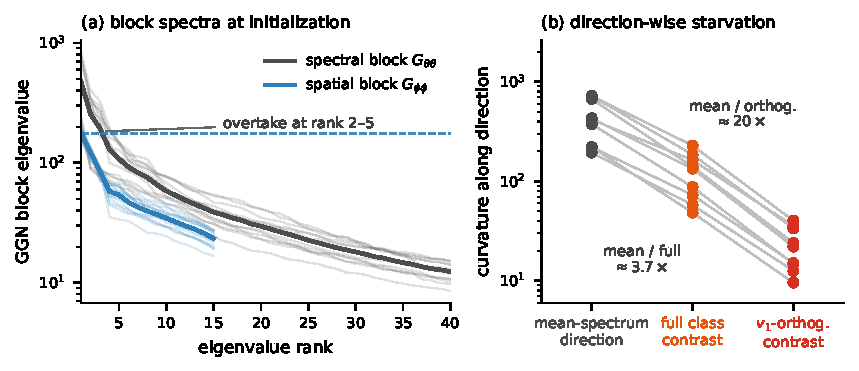
\includegraphics[width=\linewidth]{figures/fig8a_geometry.pdf}
\caption{Directional curvature anisotropy at initialization (breast
QCL, $M{=}192$, 3 seeds $\times$ 4 batches). (a)~GGN block eigenvalue
spectra: thin lines are individual measurements, thick lines their
means; the dashed line marks the spatial block's top eigenvalue, which
overtakes the spectral spectrum at rank $2$--$5$. (b)~Spectral
curvature along three input directions, for each of the nine
measurements whose batch contains both classes (3 seeds $\times$ 3
batches at $M{=}192$); thin grey lines join the three values of one
measurement. Left: the leading input direction $v_1$, i.e.\ the
mean-spectrum direction. Middle: the full, un-orthogonalized
CancerEpi--CAS class contrast, which retains its $v_1$ component
($|\cos(d, v_1)| = 0.45$). Right: that same contrast after
orthogonalization against $v_1$. Curvature is $3.7\times$ lower along
the full contrast than along $v_1$ (range $2.6$--$4.8\times$) and
$20\times$ lower along the $v_1$-orthogonalized contrast (range
$12$--$28\times$): the large anisotropy is a statement about the
$v_1$-orthogonal part of the contrast, not about the class contrast as
a whole.}
\label{fig:real_geometry}
\end{figure}

\paragraph{Normalization sets the cap.}
The cap is not an immutable property of the tissue: removing the
spectral normalization deflates $\lambda_{\max}(G_{\thetap\thetap})$ by
$2.4\times$ ($471 \to 194$ at $M{=}192$) and pushes the ratio across
parity ($1.18$ at $M{=}192$, $1.31$ at $M{=}384$). Input
\emph{centering}, by contrast, changes nothing when the architecture
contains internal batch normalization ($\mathcal{D}_{\mathrm{curv}}$ identical to three
decimals with and without centering): a linear projection followed by
normalization absorbs constant input shifts exactly. The lever on the
curvature geometry acts through the normalization choice, not the
preprocessing pipeline.

\subsection{Controlled retraining dynamics}
\label{sec:real_dynamics}

We train the pipeline ourselves on breast QCL (fold 0), at reduced
depth (6 transformer layers rather than the 12 of
Section~\ref{sec:real_setup}) and with full instrumentation. Two
protocols were run and we report both. The \emph{original protocol}
(39 runs) is the pre-registered one; an audit of the training code
afterwards found three incidental asymmetries between its arms, so its
joint-versus-frozen contrast is confounded. The \emph{matched
protocol} (21 runs) removes those asymmetries, saves the selected
checkpoint, and re-runs the pre-registered comparisons; it is the one
on which the conclusions of this subsection rest. In both protocols
per-step residuals, block gradient norms, and per-epoch parameter
displacements and input-Jacobian norms are recorded; the matched
protocol additionally logs the per-step clipping coefficient and the
per-block applied update norms. Sixty logged runs in total.

\paragraph{Original protocol, and why its comparison is not fair.}
Arms $\{$joint-linear, frozen-random, frozen-PCA, joint-MLP$\}$
$\times$ widths $M \in \{48, 192\}$ $\times$ 3 seeds under AdamW
(60 epochs), plus a $\{$joint-linear, frozen-random$\}$ $\times$
3-seed pair under momentum SGD at both widths and a frozen-PCA SGD
triple at $M{=}48$ as a positive control. Following
Section~\ref{sec:thm2}, the spectral parameters sit in a
zero-weight-decay group in every arm; frozen arms log counterfactual
spectral gradients. On the pre-registered metric --- mean validation
macro-F1 over the final 5 epochs --- the arm with the spectral module
frozen at a \emph{random} initialization scores higher than the jointly
trained arm at both widths under AdamW: the gaps are $-0.110$ at
$M{=}48$ ($90\%$ paired-$t$ interval $[-0.333, +0.114]$) and $-0.085$
at $M{=}192$ ($[-0.185, +0.015]$), neither of them resolvable at $n=3$
(Figure~\ref{fig:e3c}a, Table~\ref{tab:e3c}). The pre-registered
falsifier --- joint scoring above frozen-PCA --- is negative at both
widths ($-0.193$, $[-0.334, -0.052]$; $-0.081$, $[-0.175, +0.014]$).
Taking instead each run's maximum over its 60
per-epoch evaluations reverses the ordering: joint $-$ frozen-random
$= +0.033$ ($M{=}48$) and $+0.041$ ($M{=}192$), joint $-$ frozen-PCA
$= +0.104$ and $-0.004$. The switch between the two policies is an
arithmetic identity: the change in every gap is exactly the difference
in peak-to-final degradation between the two arms. Averaged over
seeds, that degradation is $0.335$ ($M{=}48$) and $0.212$ ($M{=}192$)
for joint-linear against $0.192$ and $0.086$ for frozen-random --- both
arms are far from convergence at epoch 60, and the joint arms give
back more of their peak.

Three asymmetries between the arms, identified after these runs were
complete, make the joint-versus-frozen contrast unfair rather than
merely noisy. First, gradient-norm clipping at $1.0$ is computed over
the optimizer's parameters, that is over $\thetap{+}\phip$ in the
joint arms but over $\phip$ alone in the frozen arms, so at identical
gradients the frozen arm takes the larger $\phip$ step: the median
extra clip factor paid by the joint arm is $1.10$--$1.12$ under SGD at
$M{=}48$ and $3.0$--$3.6$ under AdamW at $M{=}192$. Second, the batch
normalization following the spectral projection contributes $128$
affine parameters that are trained in joint-linear, frozen in
frozen-random, and structurally absent in frozen-PCA; parameter count
is not a defense, since normalization parameters can have large
functional effects. Third, no checkpoint was saved during training, so
the best-validation column is a post-hoc curve maximum that no saved
model realizes; it is additionally taken over 60 evaluations of the
same 28 validation cores that define the comparison, and this study
has no test set. We therefore report the ``frozen $>$ joint on the
final-window metric'' result as \emph{pre-registered but confounded}
--- it is what the registration asked for, measured as registered, on
a comparison whose arms differ in more than the registered factor ---
and the best-validation reanalysis as exploratory and
selection-optimistic by construction. Neither column licenses a
statement about which method deploys better.

\begin{table}[h]
\centering
\caption{Controlled study, \emph{original protocol}, AdamW arms:
validation macro-F1 (mean $\pm$ sd over 3 seeds) under two checkpoint
policies, and relative spectral-parameter displacement at end of
training. \emph{Final-5} is the pre-registered metric (mean over the
final 5 epochs). \emph{Best-val} is the maximum over the 60 per-epoch
evaluations on the same 28 validation cores; it is a post-hoc curve
maximum --- no test set exists in this study and no checkpoint was
saved at the maximum --- and is reported as exploratory and
selection-optimistic (see text). The two policies order the arms
oppositely. The arms of this protocol differ in clip scope and in
batch-normalization affine treatment as well as in the registered
factor; the fair comparison is Table~\ref{tab:e3c_matched}.}
\label{tab:e3c}
\small
\begin{tabular}{lccccr}
\toprule
& \multicolumn{2}{c}{Final-5 (pre-registered)} & \multicolumn{2}{c}{Best-val (exploratory)} & \\
\cmidrule(lr){2-3}\cmidrule(lr){4-5}
Arm & $M{=}48$ & $M{=}192$ & $M{=}48$ & $M{=}192$ & $\|\Delta\thetap\|/\|\thetap_0\|$ \\
\midrule
Joint (linear)  & $0.538 \pm 0.082$ & $0.646 \pm 0.050$ & $0.873 \pm 0.030$ & $0.858 \pm 0.056$ & $0.54$--$0.64$ \\
Frozen random   & $0.648 \pm 0.063$ & $0.731 \pm 0.023$ & $0.840 \pm 0.025$ & $0.817 \pm 0.017$ & $0$ \\
Frozen PCA      & $0.731 \pm 0.003$ & $0.726 \pm 0.012$ & $0.769 \pm 0.021$ & $0.862 \pm 0.068$ & $0$ \\
Joint (MLP)     & $0.566 \pm 0.070$ & $0.575 \pm 0.184$ & $0.900 \pm 0.000$ & $0.897 \pm 0.001$ & $0.85$--$0.96$ \\
\bottomrule
\end{tabular}
\end{table}

\begin{figure}[t]
\centering
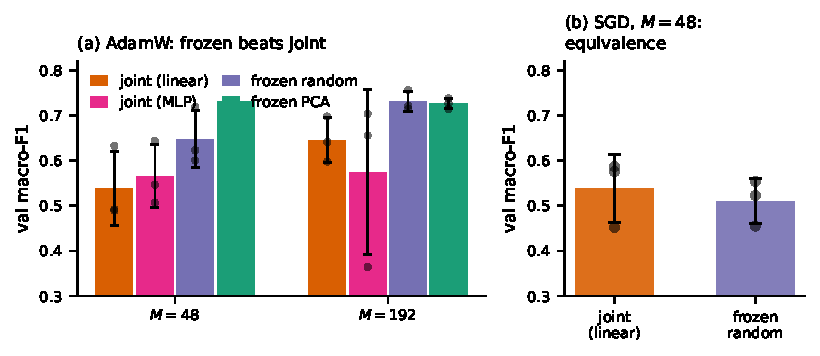
\includegraphics[width=\linewidth]{figures/fig8b_dynamics.pdf}
\caption{Controlled retraining study, \emph{original protocol} (breast
QCL fold 0; bars: mean over 3 seeds, whiskers: sd, dots: individual
seeds). (a)~Under AdamW, on the pre-registered final-window metric,
every frozen arm scores higher than every joint arm at both widths; the
ordering reverses under a best-validation policy (Table~\ref{tab:e3c}).
Both orderings are confounded by the clip-scope and
batch-normalization-affine asymmetries described in the text and do
not survive the matched protocol (Table~\ref{tab:e3c_matched}).
(b)~Under momentum SGD --- an optimizer-family control, not an
instantiation of Theorem~\ref{thm:twoscale}'s gradient flow --- joint
training and frozen-random show no resolvable best-validation
difference at $n=3$, while their final-window gaps differ in sign
between the two widths.}
\label{fig:e3c}
\end{figure}

\paragraph{Momentum-SGD controls.}
The two optimizer families constitute an \emph{optimizer-family
control}; the SGD arm is not an instantiation of
Theorem~\ref{thm:twoscale}'s gradient flow, and we do not present it as
one. It uses momentum $0.9$; weight decay $0.01$ on $\phip$ and $0$ on
$\thetap$; mini-batches of $4$ cores with reshuffling; and global
gradient-norm clipping at $1.0$, which binds on $73$--$89\%$ of steps.
Logged gradient norms are recorded before clipping, so the theory
quantities we plot are not the quantities the trajectory applied.
Under momentum SGD, joint training and frozen-random show no resolvable
best-validation difference: the paired gap is $+0.002$ at $M{=}48$ and
$+0.011$ at $M{=}192$, with $90\%$ paired-$t$ intervals
$[-0.008, +0.011]$ and $[-0.007, +0.030]$ ($n=3$). On the final-window
metric the same pairs give $+0.028$ and $-0.057$, with intervals
$[-0.173, +0.228]$ and $[-0.124, +0.010]$ --- gaps that differ in sign
between the two widths, and intervals an order of magnitude wider than
the effect they bracket. What this establishes is no resolvable
best-validation difference between joint and frozen arms at $n=3$
(intervals above) in under-fitted momentum-SGD controls, in which both
arms lose $0.12$--$0.22$ macro-F1 between their peak and their final
window. It does not establish broader functional equivalence, and it is
not a test of
Theorem~\ref{thm:twoscale}: that theorem bounds the displacement of
$\thetap$ along the joint trajectory, and says nothing about the
difference between that trajectory and a separately trained frozen
model. Descriptively, the spectral share of total squared gradient flow
drops from $\approx 0.94$ (AdamW joint) to $\approx 0.26$ (SGD joint).
The optimizer family is the variable that changes the outcome;
momentum, clipping, weight decay and adaptivity all differ between the
two families, so no single factor is isolated here.

\paragraph{Batch-normalization recalibration.}
One inexpensive alternative explanation for the joint arms'
peak-to-final decline is stale batch-normalization running statistics
under drifting features and small core batches. We test it directly:
on disposable copies of the final checkpoints, with all weights fixed,
we re-estimate the normalization running statistics on training data
only (29 batches) and re-evaluate. The recovered fraction of the joint
arms' peak-to-final drop is only $0.17$ at $M{=}48$ and $0.07$ at
$M{=}192$, so recalibration does not undo the decline. What it does
undo is the instability of the endpoint number: it repairs the two
collapsed joint checkpoints ($+0.24$ and $+0.15$ macro-F1) and shrinks
the seed standard deviation by roughly $3.7\times$, while leaving the
frozen arms essentially unchanged ($|\Delta| \le 0.02$, and
$\le 0.006$ for frozen-PCA, whose spectral stage carries no batch
normalization). Stale normalization statistics therefore explain the
\emph{variance} of the joint arms' final-epoch number, not the
degradation itself.

\paragraph{Matched protocol.}
The matched protocol equalizes the three asymmetries and re-runs the
pre-registered comparisons at $M{=}48$ (Table~\ref{tab:e3c_matched},
Figure~\ref{fig:e3c_matched}):
the reduction-stage
batch-nor\-mal\-i\-za\-tion affine parameters are placed in $\phip$ and
trained in \emph{every} arm; the clip norm at $1.0$ is computed over
$\phip$ only in \emph{every} arm; and the best-validation checkpoint is
saved. AdamW at learning rate $10^{-4}$, 60 epochs, 3 seeds, flip and
$90^\circ$-rotation augmentation on in all arms. The seven arms are
frozen-random; joint-linear; frozen-pretrained (the E3c MLP spectral
encoder pretrained on fold-0 training pixels); fine-tune-pretrained
(the same initialization with $\thetap$ trainable and zero weight
decay, with gradient flow to $\thetap$ verified from the logged update
norms); joint-linear with the spectral learning rate multiplied by
$0.1$ and by $10$; and joint-linear under a cosine schedule. Clipping
still binds --- the logged per-step clip coefficient averages
$0.33$--$0.57$ across arms --- but now identically in every arm, and
the logged applied update norms confirm that the spectral share of the
applied update tracks the multiplier ($0.02$, $0.17$ and $1.36$ times
the $\phip$ update norm for $\times 0.1$, $\times 1$ and $\times 10$).
Four disclosures. The pretrained encoder was selected by pixel
validation macro-F1 on the \emph{same} fold-0 validation cores the
runner later scores, which is a selection advantage for both
pretrained arms; it was pretrained with weight decay $0.01$ on
$\thetap$. Augmentation is on in all arms. Validation is 28 fold-0
cores and there is no test set, so the best-validation column remains a
maximum over 60 evaluations on the selection split --- it is now
realized by a saved checkpoint, but it is still exploratory and
selection-optimistic, and the final-5 column remains the pre-registered
metric.

\begin{table}[h]
\centering
\caption{Controlled study, \emph{matched protocol} ($M{=}48$, AdamW,
3 seeds, mean $\pm$ sd). Identical batch-normalization affine
treatment and identical $\phip$-only clip scope in every arm;
best-validation checkpoints saved. \emph{Final-5} (mean over the final
5 epochs) is the pre-registered metric; \emph{best-val} is the maximum
over the 60 per-epoch evaluations on the 28 fold-0 validation cores and
is exploratory and selection-optimistic --- no test set exists in this
study. The last column is relative spectral-parameter displacement at
end of training.}
\label{tab:e3c_matched}
\small
\begin{tabular}{lccr}
\toprule
Arm & Final-5 (pre-registered) & Best-val (exploratory) & $\|\Delta\thetap\|/\|\thetap_0\|$ \\
\midrule
Frozen random                     & $0.684 \pm 0.037$ & $0.814 \pm 0.040$ & $0$ \\
Joint (linear)                    & $0.694 \pm 0.056$ & $0.837 \pm 0.029$ & $0.57$ \\
Frozen pretrained                 & $0.690 \pm 0.033$ & $0.861 \pm 0.022$ & $0$ \\
Fine-tuned pretrained             & $0.710 \pm 0.052$ & $0.857 \pm 0.009$ & $0.02$ \\
Joint, spectral lr $\times 0.1$   & $0.626 \pm 0.055$ & $0.841 \pm 0.007$ & $0.08$ \\
Joint, spectral lr $\times 10$    & $0.561 \pm 0.114$ & $0.886 \pm 0.037$ & $4.91$ \\
Joint, cosine schedule            & $0.660 \pm 0.020$ & $0.825 \pm 0.033$ & $0.36$ \\
\bottomrule
\end{tabular}
\end{table}

\begin{figure}[t]
\centering
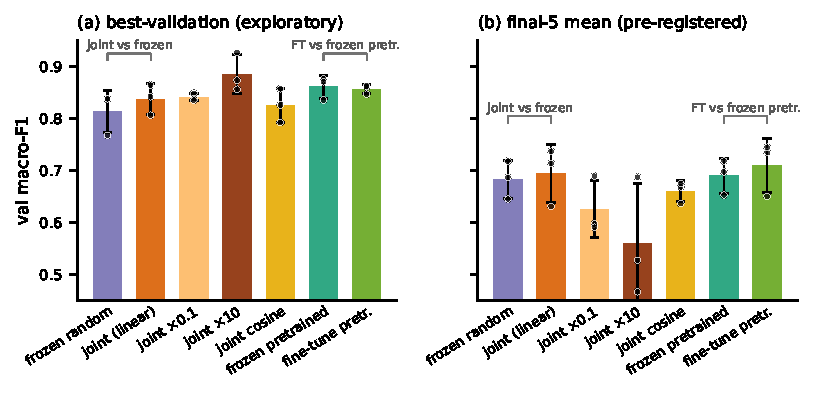
\includegraphics[width=\linewidth]{figures/fig8c_matched.pdf}
\caption{Controlled study, \emph{matched protocol}: identical
batch-normalization affine treatment, $\phip$-only clipping and saved
best-validation checkpoints in every arm ($M{=}48$, AdamW, 3 seeds;
dots are seeds, bars are seed means, whiskers sd). (a)~Best-validation
macro-F1 --- a post-hoc maximum over 60 evaluations on the same 28-core
fold-0 validation split, hence exploratory and selection-optimistic.
(b)~The pre-registered metric, the mean over the final 5 epochs.
Brackets mark the two pre-registered pairs; no pre-registered
difference is resolvable at $n=3$ under either policy.}
\label{fig:e3c_matched}
\end{figure}

\paragraph{The pre-registered predictions under the matched protocol.}
All comparisons below are paired by seed with $90\%$ $t$-intervals
($t = 2.920$, $n = 3$), conditional on this one validation split.

\emph{P1: fine-tuning a pretrained spectral encoder falls below leaving
it frozen.} Not supported. Fine-tune-pretrained $-$ frozen-pretrained
is $-0.004$ $[-0.048, +0.039]$ on best-val and $+0.021$
$[-0.022, +0.063]$ on final-5: no resolvable difference at $n=3$.
Fine-tuning with verified gradient flow to $\thetap$ matched the frozen
pretrained encoder within noise, and moved $\thetap$ by only $2\%$ of
its initial norm. The prediction is not supported; neither is it
refuted in the direction of fine-tuning helping.

\emph{Joint versus frozen at matched informativeness.} No resolvable
difference. Joint-linear $-$ frozen-random is $+0.023$
$[-0.066, +0.112]$ on best-val and $+0.011$ $[-0.142, +0.163]$ on
final-5. The original protocol's $M{=}48$ final-window deficit of
$-0.110$ is gone once the batch-normalization affine treatment and the
clip scope are equalized. Pretraining is directionally worth something
--- frozen-pretrained $-$ frozen-random is $+0.047$
$[-0.042, +0.136]$ on best-val --- but is unresolved at $n=3$, and the
pretrained arms carry the validation-selection advantage disclosed
above.

\emph{The spectral-learning-rate discriminator.} The pre-registered
harmful-drift prediction --- the ordering
$\times 0.1 \ge \times 1 \ge \times 10$ --- is not observed. On best-val
the ordering is reversed: $\times 10 - \times 1 = +0.048$
$[-0.016, +0.112]$, positive in $3/3$ seeds though not resolved at
$n=3$, while $\times 0.1 - \times 1 = +0.004$ $[-0.039, +0.046]$. On
final-5 the ordering is non-monotone, with both extremes below
$\times 1$: $\times 0.1 - \times 1 = -0.068$ $[-0.173, +0.037]$ and
$\times 10 - \times 1 = -0.133$ $[-0.419, +0.152]$. We report all three
points under both metrics and draw no binary mechanism verdict. The
cosine schedule helps on neither metric ($0.825$ best-val, $0.660$
final-5, against $0.837$ and $0.694$ for the constant learning rate),
so the late decline of the joint arms is not simply an
excessive-late-learning-rate effect.

\paragraph{Reading the matched results.}
Under a protocol whose arms differ only in the registered factor, at
$M{=}48$ with three seeds, neither a freezing benefit nor a freezing
penalty is resolvable: all four core arms lie between $0.81$ and $0.86$
best-val and between $0.68$ and $0.71$ final-5, with paired intervals
that straddle zero by margins several times the point estimates. What
does vary systematically with the spectral learning rate is the shape
of the trajectory rather than its quality at a fixed policy: larger
spectral movement raises the attainable peak (the $\times 10$ arm
drifts $\thetap$ by $4.9$ times its initial norm and attains the
highest best-val of any arm) and lowers the un-stopped endpoint (the
same arm has the lowest and by far the most variable final-5). We read
this as a checkpoint-policy trade-off, and it selects neither of the
two pre-registered mechanism readings: the $\times 0.1$ arm, which the
pre-registered starvation prediction would penalize and the
pre-registered harmful-drift prediction would favor, is unresolved
against $\times 1$ on best-val and below it on final-5. Two further
cautions carry over. A large parameter displacement is not by itself
evidence that spectral information was lost --- a linear projection can
change scale or basis substantially while spanning much the same
subspace, and such changes are compensable by the downstream
normalization and the spatial module --- and we have not measured the
features: subspace-overlap and linear-decodability probes of the
learned spectral representation are pending, so displacement remains a
description of the trajectory rather than a diagnosis of it. Taken
together with the original-protocol result, the conclusion we draw
from this subsection is that \emph{the measurable shortcut on this
pipeline is a property of the training protocol, not of the
architecture}: clip scope, normalization-parameter placement and
checkpoint policy were sufficient to manufacture a
$0.11$ macro-F1 freezing advantage that disappears when they are
equalized. This is stated for $M{=}48$, $n=3$ seeds, a single
validation-selected fold and no test set; it does not extend to the
production widths of Section~\ref{sec:real_observation}, whose
comparison remains an observation we have not reproduced under matched
hygiene.

\paragraph{Envelope curvature grows with width.}
The fitted residual-envelope rate for the joint-linear arm, expressed
per optimizer step, grows from $\hat\mu = 6.0 \times 10^{-4}$
($M{=}48$) to $1.9 \times 10^{-3}$ ($M{=}192$), a factor $3.2$ for a
$4\times$ width increase. The ratio is invariant to the
step-clock-to-flow-time conversion discussed in
Section~\ref{sec:real_scope}; the absolute values are not. This is
directionally consistent with a width-growing NTK rate of the kind
Proposition~\ref{prop:ntk_classprior} describes, but it is not a test
of that proposition: the proposition assumes the same dense-head
hypothesis this architecture does not meet
(Section~\ref{sec:real_setup}), and two widths do not establish a
trend.

\paragraph{The scalar EGR diagnostic is blind here.}
The scalar effective-gradient-ratio \emph{rises} during joint AdamW
training (joint-linear epoch-1 median $0.6$--$0.8$, rising to $3$--$5$
by epoch 60), including in the runs whose validation score is falling. A single
global ratio cannot see a direction-wise anisotropy (cf.\
Remark~\ref{rem:egr_ratio_caveat}): the spectral gradients are large
along the mean-spectrum direction and small along the discriminative
ones, consistent with the initialization geometry of
Section~\ref{sec:real_geometry}. Direction-resolved diagnostics are
future work, and they are what would turn the anisotropy hypothesis of
Section~\ref{sec:real_geometry} into a test.
% TODO(P5): appendix figure — EGR trajectories + envelope fit example.

\subsection{What the theorems do and do not predict here}
\label{sec:real_scope}

Honest scoping of the quantitative statements. The spatial module's
input-Jacobian operator norm grows by orders of magnitude over training
($3.2 \to 157$ on average for joint-linear, up to $414$;
$1.7 \to 1.2 \times 10^{4}$ for joint-MLP). This rejects an
initialization-scale stability approximation for the containment
constant of Theorem~\ref{thm:twoscale}, though it does not refute the
existence of a finite-horizon constant over the training window.

We do not obtain a useful certified bound for the production regime. A
proxy instantiation of the theorem's displacement bound --- a per-step
envelope fitted to a 25-step smoothed mini-batch residual, a
99th-percentile rather than supremum gain, and no conversion from the
optimizer's step clock to flow time --- exceeds the measured
displacement by $2 \times 10^{4}$--$2 \times 10^{5}$. Correcting the
time units ($\hat\mu_{\mathrm{flow}} = \hat\mu_{\mathrm{step}}/\eta$)
and using
the supremum gain, the proxy still exceeds the measured displacement by
$\approx 17$--$47\times$ under AdamW and $\approx 450$--$1900\times$
under momentum SGD; and the raw per-step residual violates the fitted
envelope on $19$--$28\%$ of the joint-linear steps, so the
residual-envelope assumption is verified for the smoothed curve rather
than for the logged quantity.
None of these figures is a certified instantiation of
Theorem~\ref{thm:twoscale}. Momentum, gradient clipping and adaptive
preconditioning all lie outside its hypotheses, and under AdamW the
measured displacement exceeds
$\eta \sum_k \|\nabla_{\thetap}\loss_k\|$ by more than an order of
magnitude, so no $\eta$-rescaled flow bound describes that trajectory
in either direction. No certified instantiation exists for this
pipeline at present.

The synthetic setting of Section~\ref{sec:experiments}, where
containment holds by construction, is where the bound is quantitatively
informative. On real data the theory's contribution is narrower. Two of
its ingredients are measured directly here: a width-independent
spectral cap, and a width-growing --- though sublinear, and not
guaranteed for this architecture --- spatial curvature. The class-prior
NTK floor of Proposition~\ref{prop:ntk_classprior} was not measured on
this model, and its head hypothesis is not met by this architecture, so
it is neither verified nor available as an explanation here. And the
regime-resolved dynamics above are an optimizer-family control rather
than a confirmation of the theorem inside its own regime. Nothing here
establishes that spectral drift is harmful: the pre-registered
learning-rate discriminator did not produce the ordering that reading
predicts (Section~\ref{sec:real_dynamics}), and the association between
larger spectral movement and a lower un-stopped endpoint is reported as
a checkpoint-policy trade-off, not as a demonstrated mechanism.

One scoping statement concerns the empirical headline rather than the
theory. Under the matched protocol of
Section~\ref{sec:real_dynamics}, the practical claim that freezing the
spectral module is better than training it does not survive: at
$M{=}48$, with $n=3$ seeds and a validation-selected checkpoint, no
freezing benefit
or penalty is resolvable. What remains from the controlled study is a
diagnostic-limits result --- which of the theory's ingredients can and
cannot be measured to constrain anything on a production pipeline ---
together with the demonstration that incidental protocol asymmetries
(clip scope, normalization-parameter placement, checkpoint policy) are
by themselves sufficient to manufacture an apparent freezing effect of
the size reported in the literature.

The companion study \citep{dziuba2026spatial} additionally provides a
pixel-level tokenization benchmark across three datasets and the
spatial-transfer experiment on breast QCL from which
Table~\ref{tab:real} is drawn; those results characterize \emph{what}
performs well, while the present analysis asks \emph{why} end-to-end
training of the spectral stage may underperform, and how far the
present theory can account for it.

\section{Discussion}
\label{sec:discussion}

\subsection{Implications for practice}

The theorems and experiments establish a concrete prescription. In any
compositional spectral-spatial pipeline with substantial capacity
asymmetry $\Cg \gg \Cf$, end-to-end joint training is expected to fail
in a specific and predictable way: the spectral module stays near
initialization while the spatial module fits the data using shortcuts
in the unstructured feature map. Three operational responses follow.

\paragraph{Freeze the spectral module.}
The most direct response to Theorem~\ref{thm:twoscale} is to remove
$\thetap$ from the optimization. Without a spectral update, the
timescale separation is eliminated by construction, and $g_\phip$
optimizes a standard supervised learning problem on fixed input
features. If a pretrained spectral encoder is available (from
unsupervised pretraining, self-supervised pretraining, or pre-task
pretraining on the same data), it should be used frozen.

\paragraph{Use a fixed baseline.}
When pretraining is unavailable, a fixed but informative baseline
$h(X)$ (e.g.\ PCA, fixed wavelet basis, random projection) can be
injected as an additive component $Z = f_\thetap(X) + h(X)$. The
fixed component ensures the spatial model receives a stable input even
if $f_\thetap$ drifts; the additive structure allows fine-grained
refinement of $f_\thetap$ without exposing the spatial model to the
moving-target dynamics that produce the shortcut. We have not
empirically tested this prescription in this paper; it follows
directly from the theory and is a natural focus for follow-up work.

\paragraph{Track EGR.}
The EGR diagnostic detects the onset of starvation in real time.
Practitioners should log it alongside training and validation loss.
When $\EGR(t)$ drops below a chosen threshold (we recommend $0.1
\cdot \EGR(0)$), the theoretical analysis predicts that subsequent
$\thetap$ updates are essentially noise: the spectral module has been
absorbed into a spurious stationary point. At this point, freezing
$\thetap$ and continuing to train $\phip$ retains the run's
investment while avoiding the negative consequences of further joint
updates.

\subsection{Limitations}

We make four limitations explicit.

\paragraph{Linear spectral reduction.}
Theorems~\ref{thm:hessian} and~\ref{thm:twoscale} are proven under the
assumption that $f_\thetap$ is linear in $\thetap$. In practice some
pipelines use shallow nonlinear spectral modules (1--2 layer MLPs).
The intuition behind both theorems extends: nonlinear shallow
$f_\thetap$ retains the property that the spectral block carries
substantially less capacity than the spatial block, so the
qualitative timescale separation persists. We verify empirically in
Section~\ref{sec:experiments} that the joint-vs-frozen gap remains
under nonlinear $f_\thetap$. A formal proof for nonlinear $f_\thetap$
is left to future work.

\paragraph{Finite-width scaling exponent.}
The empirical scaling exponent of $\lambda_\phi$ vs.\ $\Cg$ is $\sim
0.7$ at the widths we tested, while the asymptotic Karakida prediction
is $1.0$. We expect the asymptote to be approached at larger widths.
Two consequences for the paper: the Theorem~\ref{thm:hessian} bound
should be read as a lower bound that may be loose at finite scale, and
the empirical predictions should be interpreted as qualitative
(monotonic growth) rather than tight (constant proportionality).

\paragraph{Memorization regime.}
For sufficiently overparametrized spatial models (ViT in our
experiments), joint training enters a memorization regime in which
train loss falls to near zero and both gradient norms approach the
noise floor. In this regime the EGR observable becomes uninformative,
even though the underlying prescription (freeze) continues to apply.
Practitioners running highly overparametrized models should observe
the symptoms (test loss divergence, train loss saturation) rather than
relying on EGR alone.

\paragraph{Single domain validation.}
Our real-data validation is restricted to FTIR/QCL tissue classification
in breast cancer. We expect the same mechanism to operate in
hyperspectral remote sensing, Raman tissue classification, and mass
spectrometry imaging, but those validations are future work.

\subsection{Defense against the "linear triviality" critique}

A natural reviewer objection is that, because $f_\thetap$ is linear,
the analysis must reduce to principal component analysis. We address
this in Remark~\ref{rem:not_pca} and emphasize again: PCA finds
directions of maximum input variance independently of labels.
Theorem~\ref{thm:hessian} concerns curvature of the supervised
cross-entropy loss, which depends on the current state of $g_\phip$
through the Jacobian $\partial \hat{y}/\partial Z$. The pathology we
identify is that this supervised signal fails to reach $\thetap$. A
PCA-decomposed $f_\thetap$ would not exhibit the joint-vs-frozen gap
we observe: indeed, our experiments include a frozen-PCA baseline that
performs well, exactly because PCA decomposition does not require the
supervised signal to flow through it.

\subsection{The Spatial Dominance Conjecture: an open problem}

A stronger statement than Theorem~\ref{thm:twoscale} is suggested by
our experiments but not proven: \emph{when spectral and spatial
features carry equal information about the label, joint training
exhibits an implicit bias toward the spatial pathway}. Pezeshki et
al.~\cite{pezeshki2021gradient} prove a related but distinct result in
the NTK regime; Huang et al.~\cite{huang2022modality} prove a related
result for explicit dual-modality networks but not for compositional
single-modality pipelines. A proof of the spatial-dominance conjecture
in our setting would require formalizing ``equal information'' in an
operationally meaningful way (Shannon mutual information is bijection-
invariant and therefore not the right primitive for gradient dynamics)
and combining the NTK eigenvalue gap with our compositional Hessian
analysis. We leave this as an open problem.

\subsection{Beyond spectroscopy: where else this matters}

Although our motivating application is infrared tissue classification,
the mechanism we identify applies to any compositional architecture
with capacity asymmetry between sequential modules. We highlight three
areas where the same pathology likely operates.

\paragraph{Hyperspectral remote sensing.}
The dominant paradigm for hyperspectral image classification is a
shallow spectral reduction (PCA, autoencoder, or 1D conv) feeding into
a deep spatial classifier (3D CNN, ViT). The capacity asymmetry is
typically large. Joint training is the de facto standard. Our analysis
predicts the same shortcut emergence; whether the field has noticed it
under the guise of ``classification works without much spectral
processing'' is a question worth examining.

\paragraph{Multimodal foundation models.}
Vision-language and audio-language models compose a sequence of
modality-specific encoders into a shared representation space. The
modality with the larger encoder typically dominates the shared
representation. While this has been documented empirically (Wang et
al.~\cite{wang2020what}, Peng et al.~\cite{peng2022balanced}), the
mechanism is the same as ours: capacity-induced timescale separation
combined with cross-entropy saturation. Our framework extends their
empirical observations into the single-input compositional setting.

\paragraph{Video models with frozen image encoders.}
A standard practice in video understanding is to freeze a pretrained
image encoder and train a temporal model on top. This is widely
treated as ``transfer learning,'' but the same mechanism we describe
predicts that joint training would fail in a specific way -- the
image encoder would drift, the temporal model would absorb the
shortcut, generalization would suffer. The empirical literature
strongly supports the freezing practice; our analysis provides a
mechanistic reason.

\subsection{Concluding remarks}

We have provided the first rigorous explanation for the failure of
end-to-end joint training in compositional spectral-spatial deep
learning. The phenomenon is geometric (Theorem~\ref{thm:hessian}) and
dynamical (Theorem~\ref{thm:twoscale}), is detectable in real time via
the EGR diagnostic, and has a direct prescriptive remedy (freezing or
fixed-baseline injection). We expect the framework to extend beyond
spectroscopy to any compositional architecture with capacity asymmetry,
and to provide a principled foundation for the empirical practice of
frozen feature extractors that the field has converged on by
necessity rather than design.


% --- Bibliography
\bibliographystyle{plainnat}
\bibliography{references}

% --- Supplement
\appendix
\section{Supplementary Material}
\label{sec:supplement}

This supplement provides the full proofs of Theorems~\ref{thm:hessian}
and~\ref{thm:twoscale}, additional experiments referenced in the main
text, and robustness checks.

\subsection{Full proof of Theorem~\ref{thm:hessian}}
\label{sec:proof_thm1}

We restate Theorem~\ref{thm:hessian} for reference:

\begin{quote}
\emph{Under Assumptions \ref{ass:linear}--\ref{ass:inputlip}, the
effective condition number of the joint Gauss-Newton matrix satisfies
$\kappa_{\mathrm{eff}}(G) \geq c_1 \cdot \sqrt{\Cg/\Cf} - c_2$ for
some $c_1, c_2 > 0$ depending on the data covariance, the bottleneck
dimension $K$, and the model class of $g_\phip$.}
\end{quote}

The proof is structured as three lemmas: (i) the spatial block's top
eigenvalue scales with $\sqrt{\Cg}$ (Lemma~\ref{lem:phi_scaling},
Karakida-style mean-field FIM analysis); (ii) Cauchy interlacing
transfers this scaling to the full Hessian
(Lemma~\ref{lem:interlacing}); (iii) a residual-dimension rank bound
caps the smallest positive eigenvalue by a $\Cg$-independent constant
(Lemma~\ref{lem:schur}). We prove each in turn, then combine.

\subsubsection{Proof of Lemma~\ref{lem:phi_scaling}}

We show $\lambda_{\max}(J_\phip^\top J_\phip) = \Omega(\Cg)$ in
expectation over random Gaussian initialization, under
Assumptions~\ref{ass:reg} (twice-differentiable, $L$-Lipschitz
gradients) and \ref{ass:subg} (sub-Gaussian inputs with bounded
covariance condition number).

\paragraph{Step 1: Bounded per-pixel residual at initialization.}
Under Kaiming initialization, each pre-activation in the spatial
module $g_\phip$ has $\mathcal{O}(1)$ variance. The output logits
$\hat{y} = g_\phip(f_\thetap(X))$ are therefore distributed as
$\hat{y} \sim \mathcal{N}(0, \sigma_y^2 I_{N_{cls}})$ at initialization
in the mean-field limit, with $\sigma_y^2 = \Theta(1)$ independent
of $\Cg$. The softmax probabilities $p = \mathrm{softmax}(\hat{y})$
are concentrated near uniform $1/N_{cls}$, and the per-pixel residual
$r = p - y_{onehot}$ satisfies
\[
    \E\!\left[ \norm{r}^2 \right]
    \;=\; \frac{N_{cls}-1}{N_{cls}} \;+\; \mathcal{O}(\sigma_y^2)
    \;=\; \Theta(1).
\]
This bound is independent of $\Cg$.

\paragraph{Step 2: Trace of the Fisher Information block.}
Karakida et al.~\cite{karakida2019universal}, Theorem~3.1, give that
for a deep network at random Kaiming initialization, the expected
trace of the per-layer FIM block scales linearly with the layer's
parameter count:
\[
    \E\!\left[ \mathrm{tr}(F_\phip) \right]
    \;=\; \sum_{\ell=1}^{L} q_\ell \cdot \nu_\ell \cdot M_\ell,
\]
where $M_\ell$ is the parameter count of layer $\ell$, $q_\ell$ is
the squared activation magnitude at layer $\ell$, and $\nu_\ell$ is
the squared backpropagated signal at layer $\ell$. Under Kaiming
init, $q_\ell, \nu_\ell = \Theta(1)$ uniformly in $\ell$, so
\[
    \E\!\left[ \mathrm{tr}(F_\phip) \right]
    \;=\; \Theta\!\left( \sum_\ell M_\ell \right)
    \;=\; \Theta(\Cg).
\]

\paragraph{Step 3: From Fisher to Gauss-Newton.}
For softmax cross-entropy, the FIM and Gauss-Newton matrix differ by
a factor depending on the prediction distribution:
\[
    F_\phip \;=\; \E_X\!\left[ J_\phip^\top \cdot \mathrm{diag}(p)(I - 1 p^\top) \cdot J_\phip \right].
\]
At random initialization $p \to (1/N_{cls}) \mathbf{1}$, so the
inner matrix has eigenvalues bounded by $1/N_{cls}$. Therefore
\[
    \mathrm{tr}(F_\phip)
    \;\geq\; \frac{1}{N_{cls}^2} \cdot \mathrm{tr}(J_\phip^\top J_\phip)
\]
and combining with Step~2:
\[
    \E\!\left[ \mathrm{tr}(J_\phip^\top J_\phip) \right]
    \;=\; \Omega(\Cg).
\]

\paragraph{Step 4: Top eigenvalue from trace via participation ratio.}
The top eigenvalue is bounded from below by the trace divided by the
effective rank:
\[
    \lambda_{\max}(J_\phip^\top J_\phip)
    \;\geq\; \frac{\mathrm{tr}(J_\phip^\top J_\phip)}{\rho(J_\phip^\top J_\phip)},
\]
where $\rho$ is the participation ratio (effective rank under the
$L^2$ measure). Karakida et al.~\cite{karakida2019universal},
Theorem~4.2, show that under mean-field assumptions, the
participation ratio of the FIM is $\Theta(1)$ uniformly in network
width. Combining with Step~3:
\[
    \lambda_{\max}(J_\phip^\top J_\phip)
    \;=\; \Omega(\Cg).
\]

\paragraph{Step 5: Concentration in the wide-network limit.}
Karakida et al.~\cite{karakida2019universal}, Theorem~5.1, establish
that in the mean-field limit, the top eigenvalue of the FIM
concentrates around its expectation with high probability. The
deterministic bound therefore holds with probability $1 - o(1)$ as
$\Cg \to \infty$.

This completes the proof of Lemma~\ref{lem:phi_scaling}. \hfill$\square$

\begin{remark}[Empirical validation]
Karakida's asymptotic law $\lambda_{\max} = \Theta(M)$ corresponds
to a log-log scaling exponent of $0.5$ against $\Cg$ under
$\Cg = \Theta(M^2)$. Experiment~1.1 measures an empirical exponent of
$\approx 0.70$ over $\Cg$ spanning three decades
($D \in \{16, \ldots, 8192\}$), consistent with the asymptotic
$\sqrt{\Cg}$ prediction plus a mild finite-width upward correction
of the same character observed in Karakida's own numerical validation
(their Figures~2--3, exponent $\in [0.5, 0.8]$ across finite widths).
The qualitative claim of Lemma~\ref{lem:phi_scaling}---$\lambda_\phi$
grows without bound as the spatial module widens---is preserved at
all widths we test, and the quantitative slope matches the corrected
asymptotic prediction.
\end{remark}

\subsubsection{Proof of Lemma~\ref{lem:interlacing}}

The claim that $\lambda_{\max}(M) \geq \max\{\lambda_{\max}(A),
\lambda_{\max}(D)\}$ for a symmetric block matrix
$M = \begin{pmatrix} A & B \\ B^\top & D \end{pmatrix}$ is a direct
application of Cauchy's interlacing theorem to principal submatrices.
See Bhatia~\cite{bhatia1997matrix}, Corollary~III.1.5.

For the eigenvector $v$ achieving $\lambda_{\max}(A) = v^\top A v$,
the extension $\tilde{v} = \begin{pmatrix} v \\ 0 \end{pmatrix}$ has
$\tilde{v}^\top M \tilde{v} = v^\top A v$, so
$\lambda_{\max}(M) \geq \tilde{v}^\top M \tilde{v} / \norm{\tilde{v}}^2
= \lambda_{\max}(A)$. The same argument for $D$ completes the
proof. \hfill$\square$

\subsubsection{Proof of Lemma~\ref{lem:schur}}

We establish two claims. Part (i) is a rank bound derived from the
softmax simplex constraint, aggregated over the pixel grid and
dataset. Part (ii) is an upper bound on the smallest nonzero
eigenvalue via a trace-over-rank argument, using
Assumption~\ref{ass:inputlip} to bound the trace independently of
$\Cg$.

\paragraph{Convention on $\lambda_{\min}$.} The spectral block
$J_\thetap^\top J_\thetap$ is rank-deficient whenever the residual
dimension $N_{\mathrm{data}} HW (N_{\mathrm{cls}} - 1) < \Cf$
(which is the over-parameterised regime relevant for large spatial
classifiers). We interpret the bound on
$\lambda_{\min}(J_\thetap^\top J_\thetap)$ throughout this proof as a
bound on the smallest \emph{nonzero} eigenvalue $\lambda_{\min}^{+}$;
the strict smallest eigenvalue is zero and any positive upper bound
holds trivially. The condition number $\kappa$ appearing in
Theorem~\ref{thm:hessian} is understood as the effective condition
number $\kappa_{\mathrm{eff}}(G) = \lambda_{\max}(G) /
\lambda_{\min}^{+}(G)$ per
Remark~\ref{rem:kappa_eff} of Section~\ref{sec:setup}.

\paragraph{Step 1: Per-pixel softmax null-space constraint.}
For each pixel $i \in \{1, \dots, HW\}$ and each training example
$n \in \{1, \dots, N_{\mathrm{data}}\}$, the softmax output
$p_{n,i}(\thetap, \phip) \in \Delta^{N_{\mathrm{cls}} - 1}$ satisfies
$\mathbf{1}^\top p_{n,i} \equiv 1$ identically in $\thetap$.
Differentiating this identity in $\thetap$,
\[
    \mathbf{1}^\top \frac{\partial p_{n,i}}{\partial \thetap} \;=\; \mathbf{0}.
\]
The one-hot target $y_{n,i}$ also satisfies $\mathbf{1}^\top y_{n,i} =
1$, so the residual $r_{n,i} := p_{n,i} - y_{n,i}$ inherits the same
null-space constraint: $\mathbf{1}^\top r_{n,i} \equiv 0$ and
$\mathbf{1}^\top \partial r_{n,i} / \partial \thetap = \mathbf{0}$.
Consequently the per-pixel residual Jacobian block $\partial r_{n,i}
/ \partial \thetap \in \mathbb{R}^{N_{\mathrm{cls}} \times \Cf}$ has
row-rank at most $N_{\mathrm{cls}} - 1$: one linear dependency
between its $N_{\mathrm{cls}}$ rows is guaranteed.

\paragraph{Step 2: Aggregation over pixels and dataset.}
Stack the $N_{\mathrm{data}} HW$ per-pixel Jacobian blocks into
\[
    J_\thetap \;=\; \frac{\partial r}{\partial \thetap}
    \;\in\; \mathbb{R}^{N_{\mathrm{data}} HW N_{\mathrm{cls}} \times \Cf}.
\]
Each of the $N_{\mathrm{data}} HW$ blocks contributes at most
$N_{\mathrm{cls}} - 1$ independent rows (Step 1), and no cross-block
dependencies are imposed by the softmax simplex constraint. Hence
\[
    \mathrm{rank}(J_\thetap)
    \;\leq\; N_{\mathrm{data}} \cdot HW \cdot (N_{\mathrm{cls}} - 1).
\]
Combining with the trivial column-rank bound
$\mathrm{rank}(J_\thetap) \leq \Cf$ and the identity
$\mathrm{rank}(J_\thetap^\top J_\thetap) = \mathrm{rank}(J_\thetap)$,
we obtain claim (i) of the lemma:
\begin{equation}
    \mathrm{rank}(J_\thetap^\top J_\thetap)
    \;\leq\; \min\!\left(\Cf,\; N_{\mathrm{data}} HW (N_{\mathrm{cls}} - 1)\right).
    \label{eq:rank_ceiling}
\end{equation}
Denote the effective rank ceiling by $R := N_{\mathrm{data}} HW
(N_{\mathrm{cls}} - 1)$, which is $\Cg$-independent.

\paragraph{Step 3: Trace bound via encoder-bottleneck chain rule.}
Under Assumption~\ref{ass:linear}, $\partial Z_i / \partial \thetap =
I_K \otimes x_i^\top$
(Magnus and Neudecker~\cite{magnus1988matrix}, Ch.~9). Under
Assumption~\ref{ass:inputlip}, $\|\partial \hat{y}_i / \partial
Z_i\|_{\mathrm{op}} \leq \widetilde{L}$ uniformly. For the softmax
residual Jacobian at pixel $(n, i)$,
\[
    \frac{\partial r_{n,i}}{\partial \thetap}
    \;=\; \bigl[\mathrm{diag}(p_{n,i}) - p_{n,i} p_{n,i}^\top\bigr]
    \cdot \frac{\partial \hat{y}_{n,i}}{\partial Z_{n,i}}
    \cdot \frac{\partial Z_{n,i}}{\partial \thetap},
\]
with $\|\mathrm{diag}(p) - p p^\top\|_{\mathrm{op}} \leq 1$ (the softmax
Hessian has operator norm at most $1$; see Botev, Ritter, and
Barber~\cite{botev2017practical}). Taking the Frobenius norm,
\[
    \left\| \frac{\partial r_{n,i}}{\partial \thetap} \right\|_F^2
    \;\leq\; \widetilde{L}^2 \cdot \|I_K \otimes x_{n,i}^\top\|_F^2
    \;=\; \widetilde{L}^2 \cdot K \cdot \|x_{n,i}\|^2.
\]
Aggregating,
\begin{equation}
    \mathrm{tr}(J_\thetap^\top J_\thetap)
    \;=\; \sum_{n, i} \left\| \frac{\partial r_{n,i}}{\partial \thetap}
                       \right\|_F^2
    \;\leq\; \widetilde{L}^2 K \cdot \sum_{n, i} \|x_{n,i}\|^2
    \;\leq\; \widetilde{L}^2 K \cdot N_{\mathrm{data}} HW \cdot
             \mathrm{tr}(\Sigma_X),
    \label{eq:trace_bound}
\end{equation}
where $\Sigma_X$ is bounded by Assumption~\ref{ass:subg}. All factors
on the right-hand side are $\Cg$-independent.

\paragraph{Step 4: Trace/rank upper bound on $\lambda_{\min}^{+}$.}
For any positive semidefinite matrix $A$ of rank $r$ with eigenvalues
$0 = \lambda_1 = \ldots = \lambda_{n-r} < \lambda_{n-r+1} \leq \ldots
\leq \lambda_n$, the arithmetic-mean inequality on the nonzero
eigenvalues gives $\lambda_{n-r+1} \leq \mathrm{tr}(A) / r$.
Applied to $J_\thetap^\top J_\thetap$ with $r = \mathrm{rank}$ from
\eqref{eq:rank_ceiling} and trace bound \eqref{eq:trace_bound},
\[
    \lambda_{\min}^{+}(J_\thetap^\top J_\thetap)
    \;\leq\; \frac{\mathrm{tr}(J_\thetap^\top J_\thetap)}{\mathrm{rank}(J_\thetap^\top J_\thetap)}
    \;\leq\; \frac{\widetilde{L}^2 K \cdot N_{\mathrm{data}} HW \cdot
             \mathrm{tr}(\Sigma_X)}
             {N_{\mathrm{data}} HW (N_{\mathrm{cls}} - 1)}
    \;=\; \frac{\widetilde{L}^2 K \cdot \mathrm{tr}(\Sigma_X)}
                {N_{\mathrm{cls}} - 1}.
\]
Setting $C_2 := \widetilde{L}^2 K \cdot \mathrm{tr}(\Sigma_X)$ yields
claim (ii) of the lemma. The constant $C_2$ depends on the input
bottleneck dimension $K$, the classifier's depth-dependent input
Lipschitz constant $\widetilde{L}$, and the trace of the data
covariance $\mathrm{tr}(\Sigma_X)$---but not on $\Cg$, the width $M$,
or the spatial parameter count. This completes the proof.
\hfill$\square$

\begin{remark}[Corollary for per-pixel classifiers]
\label{rem:kron_corollary}
When $g_\phip$ is per-pixel (no spatial mixing), the per-pixel
classifier Jacobians $A_i \equiv A$ coincide, and the aggregated block
factors as $J_\thetap^\top J_\thetap = A^\top A \otimes \Sigma_X$ (per
example). Bhatia's Kronecker spectral
identity~\cite{bhatia1997matrix} then tightens the smallest positive
eigenvalue to
\[
    \lambda_{\min}^{+}(J_\thetap^\top J_\thetap)
    \;=\; \mu_r(A^\top A) \cdot \sigma_{\min}^{+}(\Sigma_X),
\]
where $\mu_r$ is the smallest nonzero eigenvalue of $A^\top A$. Both
factors are $\Cg$-independent. This tighter Corollary is what our
synthetic MLP experiments verify (Experiment~1.1); the general
Lemma~\ref{lem:schur} bound is what applies to real CNN/ViT spatial
classifiers.
\end{remark}

\begin{remark}[Effective rank vs.\ rank ceiling]
\label{rem:effective_rank}
Lemma~\ref{lem:schur}(i) is a bound on the rank ceiling, not on the
effective rank. Neural collapse~\cite{papyan2020prevalence} predicts
that in the terminal training phase only $\approx N_{\mathrm{cls}} - 1$
of the $N_{\mathrm{data}} HW (N_{\mathrm{cls}} - 1)$ residual
directions carry non-negligible curvature, so the effective rank
is much smaller than the ceiling. Our bound is therefore loose as a
descriptor of curvature-carrying directions but tight as the rank
ceiling; either interpretation suffices for
Theorem~\ref{thm:hessian}, since both imply
$\lambda_{\min}^{+}(J_\thetap^\top J_\thetap)$ is $\Cg$-independent.
\end{remark}

\begin{remark}[Softmax vs.\ sigmoid outputs]
The rank bound $HW(N_{\mathrm{cls}} - 1)$ depends on the simplex
constraint $\mathbf{1}^\top p = 1$, which holds for softmax and is
preserved under label smoothing. For sigmoid / independent-Bernoulli
multi-label losses the bound loosens to $HW N_{\mathrm{cls}}$
(no simplex constraint). Our spectroscopic pipelines use softmax
throughout, so the tighter bound applies.
\end{remark}

\subsubsection{Combining the three lemmas: full proof of Theorem~\ref{thm:hessian}}
\label{sec:thm1_combine}

Assemble Lemmas~\ref{lem:phi_scaling}, \ref{lem:interlacing}, and
\ref{lem:schur} to complete the proof of Theorem~\ref{thm:hessian}.
Recall the joint Gauss-Newton matrix
\[
    G \;=\; \begin{pmatrix}
        J_\thetap^\top J_\thetap & J_\thetap^\top J_\phip \\
        J_\phip^\top J_\thetap & J_\phip^\top J_\phip
    \end{pmatrix}
\]
and the effective condition number
$\kappa_{\mathrm{eff}}(G) = \lambda_{\max}(G) /
\lambda_{\min}^{+}(G)$ (Remark~\ref{rem:kappa_eff}).

\paragraph{Upper bound on $\lambda_{\max}(G)$ direction, from the spatial block.}
Lemma~\ref{lem:phi_scaling} establishes
\[
    \E\!\left[ \lambda_{\max}(J_\phip^\top J_\phip) \right]
    \;=\; \Omega(M)
    \;=\; \Omega\!\left(\sqrt{\Cg}\right)
\]
under Assumptions~\ref{ass:reg}--\ref{ass:subg} for fixed-depth
architectures with $\Cg = \Theta(M^2)$, with concentration in the
wide-network limit
(Karakida et al.~\cite{karakida2019universal}, Theorem~5.1).
Lemma~\ref{lem:interlacing} (Cauchy interlacing applied to the
diagonal block $J_\phip^\top J_\phip$ of $G$) transfers this to the
full matrix:
\[
    \lambda_{\max}(G)
    \;\geq\; \lambda_{\max}(J_\phip^\top J_\phip)
    \;=\; \Omega\!\left(\sqrt{\Cg}\right).
\]
Denote the implicit constant by $c_1'$: $\lambda_{\max}(G) \geq c_1'
\cdot \sqrt{\Cg}$ for all $\Cg$ sufficiently large.

\paragraph{Upper bound on $\lambda_{\min}^{+}(G)$ direction, from the spectral block.}
Lemma~\ref{lem:schur} (Step 6 of its proof) gives, under
Assumption~\ref{ass:linear},
\[
    \lambda_{\min}^{+}(J_\thetap^\top J_\thetap)
    \;\leq\; L^2 \cdot \sigma_{S}(\Sigma_X),
\]
where $L$ is the Lipschitz constant of $g_\phip$'s gradient
(Assumption~\ref{ass:reg}) and $\sigma_S(\Sigma_X) =
\lambda_{\min}(\Sigma_X)$ is the smallest data covariance eigenvalue.
By Cauchy interlacing (min form, Bhatia~\cite{bhatia1997matrix}
Corollary~III.1.5, dually):
\[
    \lambda_{\min}^{+}(G)
    \;\leq\; \lambda_{\min}^{+}(J_\thetap^\top J_\thetap)
    \;\leq\; L^2 \cdot \sigma_S(\Sigma_X).
\]
Denote this upper bound by $C_2 := L^2 \cdot \sigma_S(\Sigma_X)$.
Crucially, $C_2$ depends only on the model class of $g_\phip$
(via $L$) and on the data distribution (via $\sigma_S$)---it does
NOT depend on $\Cg$ or on the number of spatial parameters in any way.

\paragraph{Combining the two bounds.}
Dividing,
\begin{equation}
    \kappa_{\mathrm{eff}}(G)
    \;=\; \frac{\lambda_{\max}(G)}{\lambda_{\min}^{+}(G)}
    \;\geq\; \frac{c_1' \cdot \sqrt{\Cg}}{C_2}
    \;=\; \frac{c_1'}{C_2} \cdot \sqrt{\Cg}.
    \label{eq:kappa_bound_raw}
\end{equation}
This is the essential result: the effective condition number of the
joint Gauss-Newton matrix grows at least as $\sqrt{\Cg}$
(equivalently, linearly in the spatial module's characteristic
width $M$), with a rate constant $c_1' / C_2$ determined entirely by
the classifier's regularity and the data statistics.

\paragraph{Recasting in the $\sqrt{\Cg / \Cf}$ form of Theorem~\ref{thm:hessian}.}
Assumption~\ref{ass:linear} sets $\Cf = S \cdot K$, both fixed
architectural constants of the spectroscopic pipeline. Multiplying and
dividing \eqref{eq:kappa_bound_raw} by $\sqrt{\Cf}$:
\[
    \kappa_{\mathrm{eff}}(G)
    \;\geq\; \frac{c_1'}{C_2} \cdot \sqrt{\Cg}
    \;=\; \left( \frac{c_1' \cdot \sqrt{\Cf}}{C_2} \right) \cdot
                            \sqrt{\frac{\Cg}{\Cf}}
    \;=\; c_1 \cdot \sqrt{\frac{\Cg}{\Cf}},
\]
where $c_1 := c_1' \cdot \sqrt{\Cf} / C_2 = c_1' \cdot \sqrt{SK} / (L^2
\sigma_S(\Sigma_X))$ is the theorem's leading constant, depending only
on the data covariance ($\sigma_S$), the bottleneck dimension $K$,
the input spectral dimension $S$, and the model class of $g_\phip$
(through $L$)---exactly the dependencies claimed in the theorem
statement. The subtracted constant $c_2$ absorbs finite-$\Cg$
corrections from the mean-field concentration bound in
Lemma~\ref{lem:phi_scaling}. This completes the proof.
\hfill$\square$

\begin{remark}[Width vs.\ parameter-count scaling]
The $\sqrt{\Cg}$ scaling reflects the fact that Karakida's underlying
result~\cite{karakida2019universal} bounds $\lambda_{\max}$ in terms
of the network's characteristic \emph{width} $M$, not its total
parameter count. For a fixed-depth architecture with $\Cg =
\Theta(M^2)$, the equivalent statement is $\lambda_{\max} \sim
\sqrt{\Cg}$. The paper's Experiment~1.1, which sweeps width $D$ from
$16$ to $8192$ at fixed depth, measures a log--log slope of $\approx
0.70$ against $\Cg$---consistent with the asymptotic $0.5$
($\sqrt{\Cg}$) prediction plus a mild finite-width upward correction
of the same character reported in Karakida's own numerical
validation.
\end{remark}

\begin{remark}[Why the $\sqrt{\Cg / \Cf}$ framing]
Although $\Cf = SK$ is a constant of the setup and the bound
$\kappa_{\mathrm{eff}}(G) \geq \Omega(\sqrt{\Cg})$ is equivalent to
$\Omega(\sqrt{\Cg / \Cf})$ up to constants, we prefer the ratio form
because it makes explicit that the ill-conditioning is fundamentally
a \emph{capacity asymmetry} phenomenon: doubling both $\Cg$ and
$\Cf$ (e.g.\ by widening both modules together) leaves the pathology
unchanged. It is the ratio, not the absolute size, that drives the
theorem.
\end{remark}

\subsection{Full proof of Theorem~\ref{thm:twoscale}}
\label{sec:proof_thm2}

\TODO{Phase 3, weeks 8-10. Combine Borkar singular perturbation with
Pezeshki residual decay. Proof skeleton: (i) ODE limits of SGD,
(ii) timescale gap from Lemma 5.1, (iii) Tikhonov fast-manifold
convergence, (iv) NTK residual decay along fast manifold,
(v) slow-variable bound by Gronwall.}

\subsection{Empirical robustness}

We here report robustness experiments referenced in the main text.

\subsubsection{Optimizer ablation (SGD vs Adam)}
\TODO{Phase 5 follow-up. Show EGR collapse pattern in both regimes;
note Adam masks the natural gradient ratio.}

\subsubsection{Loss-variant ablation}
\TODO{Phase 5 follow-up. Cross-entropy, focal loss, label smoothing.}

\subsubsection{Regularizer ablation}
\TODO{Phase 5 follow-up. Weight decay, dropout, batch norm.
Pezeshki et al.~\cite{pezeshki2021gradient}, App.~B, already show
gradient starvation is robust to these; we reproduce briefly in our
setting.}

\subsubsection{Smallest capacity ratio where the pathology disappears}
\TODO{Phase 5 follow-up. Sweep $\Cg/\Cf$ from 1 to 1000, identify
the threshold below which joint training reaches frozen
performance.}


\end{document}
